%%% Hlavní soubor. Zde se definují základní parametry a odkazuje se na ostatní části. %%%

%% Verze pro jednostranný tisk:
% Okraje: levý 40mm, pravý 25mm, horní a dolní 25mm
% (ale pozor, LaTeX si sám přidává 1in)
\documentclass[12pt,a4paper]{report}
\setlength\textwidth{145mm}
\setlength\textheight{247mm}
\setlength\oddsidemargin{15mm}
\setlength\evensidemargin{15mm}
\setlength\topmargin{0mm}
\setlength\headsep{0mm}
\setlength\headheight{0mm}
% \openright zařídí, aby následující text začínal na pravé straně knihy
\let\openright=\clearpage

% číslované subsubsection
\setcounter{secnumdepth}{3}
\setcounter{tocdepth}{3}

%% Pokud tiskneme oboustranně:
% \documentclass[12pt,a4paper,twoside,openright]{report}
% \setlength\textwidth{145mm}
% \setlength\textheight{247mm}
% \setlength\oddsidemargin{15mm}
% \setlength\evensidemargin{0mm}
% \setlength\topmargin{0mm}
% \setlength\headsep{0mm}
% \setlength\headheight{0mm}
% \let\openright=\cleardoublepage

%% Pokud používáte csLaTeX (doporučeno):
\usepackage{czech}
%% Pokud nikoliv:
%\usepackage[czech]{babel}
%\usepackage[T1]{fontenc}

%% Použité kódování znaků: obvykle latin2, cp1250 nebo utf8:
\usepackage[utf8]{inputenc}

%% Ostatní balíčky
\usepackage{graphicx}
\usepackage{amsthm}
\usepackage{amsmath}
\usepackage{color}
\usepackage{colortbl}

\definecolor{seda}{rgb}{0.7,0.7,0.7}
\newcommand{\argmax}[1]{\underset{#1}{\operatorname{arg}\,\operatorname{max}}\;}
\DeclareFontFamily{OT1}{pzc}{}
\DeclareFontShape{OT1}{pzc}{m}{it}{<-> s * [1.10] pzcmi7t}{}
\DeclareMathAlphabet{\mathpzc}{OT1}{pzc}{m}{it}

\usepackage[usenames,dvipsnames]{xcolor}



%% Zrušení odsazení odstavců
\usepackage{indentfirst}
\setlength{\parindent}{0em}
\setlength\parskip{2mm}

%% Balíček hyperref, kterým jdou vyrábět klikací odkazy v PDF,
%% ale hlavně ho používáme k uložení metadat do PDF (včetně obsahu).
%% POZOR, nezapomeňte vyplnit jméno práce a autora.
\usepackage[ps2pdf,unicode]{hyperref}   % Musí být za všemi ostatními balíčky
\hypersetup{pdftitle=Jazykové modelování pro němčinu}
\hypersetup{pdfauthor=Marek Tlustý}

%%% Drobné úpravy stylu

% Tato makra přesvědčují mírně ošklivým trikem LaTeX, aby hlavičky kapitol
% sázel příčetněji a nevynechával nad nimi spoustu místa. Směle ignorujte.
\makeatletter
\def\@makechapterhead#1{
  {\parindent \z@ \raggedright \normalfont
   \Huge\bfseries \thechapter. #1
   \par\nobreak
   \vskip 20\p@
}}
\def\@makeschapterhead#1{
  {\parindent \z@ \raggedright \normalfont
   \Huge\bfseries #1
   \par\nobreak
   \vskip 20\p@
}}
\makeatother

% Toto makro definuje kapitolu, která není očíslovaná, ale je uvedena v obsahu.
\def\chapwithtoc#1{
\chapter*{#1}
\addcontentsline{toc}{chapter}{#1}
}

\begin{document}

% Trochu volnější nastavení dělení slov, než je default.
\lefthyphenmin=2
\righthyphenmin=2

%%% Titulní strana práce

\pagestyle{empty}
\begin{center}

\large

Univerzita Karlova v Praze

\medskip

Matematicko-fyzikální fakulta

\vfill

{\bf\Large BAKALÁŘSKÁ PRÁCE}

\vfill

\centerline{\mbox{
\includegraphics[width=60mm]{./img/logo.eps}}}

\vfill
\vspace{5mm}

{\LARGE Marek Tlustý}

\vspace{15mm}

% Název práce přesně podle zadání
{\LARGE\bfseries Jazykové modelování pro němčinu}

\vfill

% Název katedry nebo ústavu, kde byla práce oficiálně zadána
% (dle Organizační struktury MFF UK)
Ústav formální a aplikované lingvistiky

\vfill

\begin{tabular}{rl}

Vedoucí bakalářské práce: & RNDr. Ondřej Bojar, Ph.D. \\
\noalign{\vspace{2mm}}
Studijní program: & Informatika \\
\noalign{\vspace{2mm}}
Studijní obor: & Obecná informatika \\
\end{tabular}

\vfill

% Zde doplňte rok
Praha 2013

\end{center}

\newpage

%%% Následuje vevázaný list -- kopie podepsaného "Zadání bakalářské práce".
%%% Toto zadání NENÍ součástí elektronické verze práce, nescanovat.

%%% Na tomto místě mohou být napsána případná poděkování (vedoucímu práce,
%%% konzultantovi, tomu, kdo zapůjčil software, literaturu apod.)

\openright

\noindent
Poděkování.
Ondřejovi Bojarovi
Rudolfovi Rosovi za identifikaci anglických klauzí.
Daniel Zeman - nbestlisty

\newpage

%%% Strana s čestným prohlášením k bakalářské práci

\vglue 0pt plus 1fill

\noindent
Prohlašuji, že jsem tuto bakalářskou práci vypracoval(a) samostatně a výhradně
s~použitím citovaných pramenů, literatury a dalších odborných zdrojů.

\medskip\noindent
Beru na~vědomí, že se na moji práci vztahují práva a povinnosti vyplývající
ze zákona č. 121/2000 Sb., autorského zákona v~platném znění, zejména skutečnost,
že Univerzita Karlova v Praze má právo na~uzavření licenční smlouvy o~užití této
práce jako školního díla podle §60 odst. 1 autorského zákona.

\vspace{10mm}

\hbox{\hbox to 0.5\hsize{%
V ........ dne ............
\hss}\hbox to 0.5\hsize{%
Podpis autora
\hss}}

\vspace{20mm}
\newpage

%%% Povinná informační strana bakalářské práce

\vbox to 0.5\vsize{
\setlength\parindent{0mm}
\setlength\parskip{5mm}

Název práce:
Jazykové modelování pro němčinu
% přesně dle zadání

Autor:
Marek Tlustý

Katedra: Ústav formální a aplikované lingvistiky % Případně Ústav:
%Název katedry či ústavu, kde byla práce oficiálně zadána
% dle Organizační struktury MFF UK

Vedoucí bakalářské práce:
RNDr. Ondřej Bojar, Ph.D.
% dle Organizační struktury MFF UK, případně plný název pracoviště mimo MFF UK

Abstrakt:
% abstrakt v rozsahu 80-200 slov; nejedná se však o opis zadání bakalářské práce

Klíčová slova:
% 3 až 5 klíčových slov
jazykové modelování, němčina, 

\vss}\nobreak\vbox to 0.49\vsize{
\setlength\parindent{0mm}
\setlength\parskip{5mm}

Title: Language Modelling for German
% přesný překlad názvu práce v angličtině

Author:
Marek Tlustý

Department:
Institute of Formal and Applied Linguistics
% dle Organizační struktury MFF UK v angličtině

Supervisor:
RNDr. Ondřej Bojar, Ph.D.
% dle Organizační struktury MFF UK, případně plný název pracoviště
% mimo MFF UK v angličtině

Abstract:
% abstrakt v rozsahu 80-200 slov v angličtině; nejedná se však o překlad
% zadání bakalářské práce

Keywords:
% 3 až 5 klíčových slov v angličtině
language modelling, German, 

\vss}

\newpage

%%% Strana s automaticky generovaným obsahem bakalářské práce. U matematických
%%% prací je přípustné, aby seznam tabulek a zkratek, existují-li, byl umístěn
%%% na začátku práce, místo na jejím konci.

\openright
\pagestyle{plain}
%\setcounter{page}{1}
\tableofcontents

%%% Jednotlivé kapitoly práce jsou pro přehlednost uloženy v samostatných souborech
%\chapter*{Úvod}
\addcontentsline{toc}{chapter}{Úvod}


%\chapter{Strojový překlad?}

obecné povídání

\section{Frázový překlad}

\section{Název druhé podkapitoly v první kapitole}


%\chapter{Název druhé kapitoly}

\section{Název první podkapitoly v druhé kapitole}

\section{Název druhé podkapitoly v druhé kapitole}



\chapter{Úvod}

\chapter{Jazykové modely}
Jazykový model se snaží charakterizovat a zachytit zákonitosti v přirozeném jazyce. K tomu je možné přistupovat z pohledu statistiky nebo z pohledu hlubší lingvistické analýzy. Statistický přístup automaticky určuje všechny parametry z velkého množství textu v daném jazyce. Tento proces se nazývá \textit{trénování modelu}. Modely opírající se hlavně o lingvistiku jsou tvořeny pravidly, která je potřeba naprogramovat ručně. Lze však využít i obou přístupů zároveň, a to například tak, že model nenecháme trénovat jenom na samotném textu, ale i na morfologických nebo jiných značkách či gramatických vztazích. Právě takovými modely se budeme zabývat.

\section{Pohled z Bayesovy věty}
Na přirozený jazyk lze nahlížet jako na množinu kontextuálních jednotek (např. vět, slov nebo jejich částí), které jsou náhodnými proměnnými s určitým rozdělením pravděpodobnosti. Například při překladu hledáme takové slovo \(B\), které s největší pravděpodobností následuje po kontextu slov \(A\). Hledáme tedy takové \(B\), které maximalizuje podmíněnou pravděpodobnost \(P(B|A)\). S využitím Bayesovy věty máme:
\begin{equation}
\argmax{B} P(B|A) = \argmax{B} \frac{P(A|B) \cdot P(B)}{P(A)} 
\end{equation}
Jmenovatel můžeme vynechat, neboť \(P(A)\) je v tuto chvíli pouze konstanta, která hledání maxima nijak neovlivní. Dostáváme tedy:
\begin{equation}
\argmax{B} P(B|A) = \argmax{B} P(A|B) \cdot P(B)
\end{equation}

\section{N-gramové modely}
N-gramové modely jsou založené na statistickém pozorování dat. Využívají například skutečnosti, že některá slova se často vyskytují v určitých dvojících (obecně n-ticích) - pro němčinu typicky třeba člen a podstatné jméno. Jistě častěji spatříme v trénovacích datech \textit{der Hund} než \textit{das Hund}. Stejně jako po slovese \textit{fragen} uvidíme předložku \textit{nach} nebo \textit{um} spíše než \textit{auf} nebo \textit{an}.

Zajímá nás, jaká je pravděpodobnost výskytu takové posloupnosti slov $w_{1},\ldots,w_{m}$. Tuto pravděpodobnost vypočítáme tak, že spočítáme výskyty všech těchto posloupností v datech a normalizujeme je velikostí dat. Trénovací data jsou ale obvykle řídká\footnote{Řídkostí dat rozumíme počet různých kombinací slov v trénovacích datech vzhledem k celkovému počtu všech možných kombinací, kterých je nesrovnatelně více.}, a proto budeme chtít pozorované vlastnosti zobecnit.

Z Bayesovy věty víme, že
\begin{equation}
P(A|B) = \frac{P(A,B)}{P(B)}
\end{equation}
odtud vyjádříme $P(A,B)$ a dostaneme
\begin{equation}
P(A,B) = P(A|B) \cdot P(B)
\end{equation}
nyní aplikujeme tento vztah na $P(w_{1},\ldots,w_{m})$ $m$-krát
\begin{equation}
P(w_{1},\ldots,w_{m}) = P(w_{1}) \cdot P(w_{2}|w_{1}) \cdot P(w_{3}|w_{1},w_{2}) \cdot \ldots \cdot P(w_{m}|w_{1},\ldots,w_{m-1})
\end{equation}
Tento postup se nazývá \textbf{pravidlo zřetězení} a díky němu můžeme pravděpodobnost $P(w_{1},\ldots,w_{m})$ modelovat postupně člen po členu (např. slovo po slově).

\textbf{Markovův předpoklad} navíc říká, že každý člen posloupnosti $w_{1},\ldots,w_{m}$ závisí jen na $k$ předchozích. Potom tedy:
\begin{equation}\label{eq:markov}
P(w_{m}|w_{1} \ldots w_{m-1}) \simeq P(w_{m}|w_{m-k}, \ldots, w_{m-1})
\end{equation}
Toto tvrzení vede k zavedení pojmu n-gram a je vlastně předpokladem pro fungování n-gramových modelů.

\textbf{N-gram} je $n$ po sobě jdoucích členů $w_{1},\ldots,w_{n}$ z dané posloupnosti $w_{1},\ldots,w_{m}$ (např. $n$ po sobě jdoucích slov ve větě). Pro $n = 1, 2, 3$ používáme označení \textit{unigram}, \textit{bigram} a \textit{trigram}.

Pravděpodobnost $P(w_{m}|w_{m-k}, \ldots, w_{m-1})$ z \eqref{eq:markov} přesně určit nelze, a proto se používá odhad maximální věrohodnosti (\textbf{MLE}):
\begin{equation}\label{eq:pmle}
P_{MLE}(w_{m}|w_{m-k}, \ldots, w_{m-1}) = \frac{count(w_{m-k}, \ldots w_{m})}{\sum_{l} count(w_{m-k},\ldots,w_{m-1}, w_{l})} =
\end{equation}
\begin{equation}\nonumber
= \frac{count(w_{m-k}, \ldots w_{m})}{count(w_{m-k},\ldots,w_{m-1})}
\end{equation}
Takto se rozdělí pravděpodobnost mezi všechny spatřené n-gramy v trénovacích datech a právě toto rozdělení pravděpodobnosti tvoří \textbf{n-gramový model}.

Problémem však stále zůstává skutečnost, že pro neviděné n-gramy v testovacích datech, dostaneme nulovou pravděpodobnost.

\section{Good-Turing vyhlazování}
\textbf{Good-Turing vyhlazování} se snaží vyhradit část rozdělení pravděpodobnosti od více frekventovaných n-gramů pro ty méně frekventované a neviděné. Používá k tomu frekvenci frekvencí n-gramů $N_r$, které se v trénovacích datech vyskytly r-krát. Tedy například pro $r=3$ je $N_3$ rovno počtu n-gramů vyskytujících se v trénovacích datech právě třikrát. 

Zajímavějším příkladem je ale $N_0$ tj. počet neviděných n-gramů. Ty nemůžeme spočítat přímo, ovšem výpočet také není nijak složitý. Stačí vzít počet všech možných n-gramů a odečíst počet n-gramů viděných. Pokud uvažujeme model slov, pak pro $n=3$, velikost slovníku 100 a počet viděných n-gramů 350\,000 je $N_0 = 100^3 - 350\,000 = 650\,000$.

Tato metoda bere n-gramy, které se vyskytly r-krát, jakoby se vyskytly r*-krát
\begin{equation}\label{eq:gtr1}
r^* = (r+1) \cdot \frac {N_{r+1}}{N_r}
\end{equation}

V jednodušší variantě se pro vhodně zvolenou konstantu $k$ pravděpodobnost n-gramu vypočítá jako:
\begin{equation}
P_{GT}(w_{1},\ldots,w_{n}) = \left\{
\begin{array}{ll}
\displaystyle \frac{r^*}{\sum_{r}r\cdot N_r} & \text{je-li $r < k$}\\
&\\
\text{MLE} & \text{jinak}
\end{array} \right.
\end{equation}

Pokud bychom počítali pravděpodobnost pro všechny n-gramy podle prvního vzorce, nejen pro $r < k$, dostaly by ty nejvíce spatřené nulovou pravděpodobnost, neboť pro ně bude $N_{r+1} = 0$. Z tohoto důvodu je potřeba vhodně volit konstantu $k$ a pro $r >= k$ počítat pravděpodobnost standardně odhadem maximální věrohodnosti (MLE), který dává dobré výsledky.

Ve složitější variantě se namísto konstanty $k$ volí funkce $S(r)$ podle zjištěných hodnot $r$ a $N_r$.
\begin{equation}\label{eq:gtr2}
r^* = (r+1) \cdot \frac {S(r+1)}{S(r)}
\end{equation}

Odhad pravděpodobnosti potom vypadá následovně:
\begin{equation}
P_{GT}(w_{1},\ldots,w_{n}) = \left\{
\begin{array}{ll}
\displaystyle \frac{N_1}{N_0 \cdot N} & \text{pro r = 0} \\
&\\
\displaystyle \frac{r^*}{\sum_{r}r\cdot N_r} & \text{jinak} 
\end{array}\right.
\end{equation}

Jedním ze způsobů určení funkce $S(r)$ je vykreslit $\log N_r$ proti $\log r$ a pomocí lineární regrese proložit přímku. Hodnoty $S(r)$ se potom určují podle této přímky. Spoustu hodnot $N_r$ je ale nulových, proto se namísto $\log N_r$ používá $\log Z_r$:
\begin{equation}
Z_r = \frac{N_r}{0.5(t-q)}
\end{equation}
kde $q$, $r$ a $t$ jsou po sobě jdoucí indexy mající $N_q$, $N_r$ a $N_t$ nenulové. Je-li $N_r$ poslední nenulová frekvence n-gramů, dosadíme $t = 2r - q$. V případě, kdy $r = 1$, bereme $N_q = N_0$.

Good-Turing vyhlazování podává dobré výsledky pro málo frekventované n-gramy, a proto se v praxi často používá. Je také výchozím nastavením SRILM toolkitu\footnote{Sada nástrojů pro jazykové modelování. V tomto toolkitu budeme také trénovat všechny n-gramové modely. Více viz (odkaz na zdroj)} při trénování n-gramových modelů. Podrobněji o Good-Turing vyhlazování píše třeba .....[x] nebo ....[y].

\section{Katz back-off n-gramové modely}
V trénovacích datech se nemusel objevit n-gram, který zrovna chceme a bez použití vyhlazování bychom dostali nulovou pravděpodobnost. V trénovacích datech ale mohl být podobný n-gram lišící se jen délkou historie. Pro získání informace od kratších n-gramů se proto využívá kombinace n-gramových modelů nižších řádů pomocí \textbf{lineární interpolace}. 

K lineární interpolaci potřebujeme vektor vah $\lambda$, pro který platí:
\begin{equation}
\forall i : 0 \leq \lambda_i \leq 1 \quad \text{a} \quad \sum_{i} \lambda_i = 1
\end{equation}
Výsledná pravděpodobnost pro trigramový model pak vypadá takto:
\begin{equation}
P(w_3|w_1, w_2) = \lambda_3 P(w_3|w_1,w_2) + \lambda_2 P(w_3|w_2) + \lambda_1 P(w_3)
\end{equation}

Vektor vah je však zatím neznámý, existují algoritmy pro jeho automatické určení - např. \textit{EM algoritmus} (viz ZDROJ).

Na podobné myšlence kombinace n-gramových modelů s různou délkou historie jsou právě založeny \textbf{back-off n-gramové modely}. Ty ovšem neurčují pravděpodobnost vždy podle všech n-gramových modelů nižších řádů, ale využívají nižší řády pouze, pokud ty vyšší neposkytují dostatečnou informaci. Začíná se u modelů s nejvyšším řádem, pokud tento n-gram nebyl spatřen, proběhne tzv. \textbf{back-off} k nižšímu řádu a n-gramu se zkrátí historie o poslední člen (např. slovo). Pokud ani tento nižší řád n-gram se zkrácenou historií nikdy neviděl, pokračuje se v back-off operacích, dokud takový řád není nalezen.

Stejně jako v případě lineární interpolace se pravděpodobnosti jednotlivých modelů musely přenásobit vahami $\lambda$, aby se stále jednalo o validní rozdělení pravděpodobnosti, musíme najít takový způsob i u této metody. Zde musíme určit složitější normalizační faktor, neboť modelů nižších řádů nebudeme využívat vždy.

\textbf{Katz back-off modely} proto odhadují pravděpodobnost n-gramu následovně:
\begin{equation}
P_{BO}(w_n|w_1, \ldots, w_{n-1}) = \left\{
\begin{array}{l}
d_{w_1, \ldots, w_n} \cdot P_{MLE}(w_1, \ldots, w_n) \quad \text{pro $count(w_1, \ldots, w_n) > k$} \\
\\
\alpha_{w_1, \ldots, w_{n-1}} \cdot P_{BO}(w_n|w_2, \ldots, w_{n-1}) \quad \text{jinak} 
\end{array}\right.
\end{equation}
kde \begin{itemize}
\item{$P_{MLE}$ označuje odhad maximální věrohodnosti zavedený ve vzorci \eqref{eq:pmle}}
\item{$k$ je nejméně důležitý parametr a často je voleno $k = 0$}
\item{$d$ je snižující parametr, který zajišťuje vyhrazení určité části pravděpodobnosti pro odhady pravděpodobností s použitím back-off operací}
\item{$\alpha$ je normalizační faktor přerozdělující zbývající část pravděpodobnosti}
\end{itemize}

Parametr $d$ je možné stanovit na základě popsaného Good-Turing vyhlazování následovně:
\begin{equation}
d_{w_1, \ldots, w_n} = \frac{count(w_1, \ldots, w_n)^*}{count(w_1, \ldots, w_n)}
\end{equation}
přičemž $count(w_1, \ldots, w_n)^*$ se spočítá dle vzorce \eqref{eq:gtr1} nebo \eqref{eq:gtr2} z Good-Turing vyhlazování.

Výpočet normalizačního faktoru $\alpha$ je o něco složitější. Nejprve zavedeme $\beta$ jako doplněk pravděpodobnosti součtu všech n-gramů s počtem výskytu (count) vyšším než $k$. $\beta$ tak bude představovat zbývající vyhrazenou část pravděpodobnosti pro (n-1)-gramy.
\begin{equation}
\beta_{w_{1}, \cdots, w_{n-1}} = 1 - \sum_{ \{\text{n-gram} | count(\text{n-gram}) > k \} } d_{w_{1}, \cdots, w_{n}} P_{MLE}(w_1, \ldots, w_n)
\end{equation}
Potom se normalizační faktor $\alpha$ vypočítá jako podíl zbývající pravděpodobnosti $\beta$ a součtu pravděpodobností n-gramů vyskytujících se nejvýše $k$-krát. Tím se zajistí vždy ještě dostatek pravděpodobnosti pro další přechod k n-gramům nižších řádů back-off operacemi.
\begin{equation}
\alpha_{w_{1}, \cdots, w_{n -1}} = \frac{\beta_{w_{1}, \cdots, w_{n -1}}}        {\sum_{ \{ \text{n-gram} | count(\text{n-gram}) \leq k \} } P_{BO}(w_n | w_{2} \cdots w_{n-1})}
\end{equation}

Back-off n-gramové modely podávají dobré výsledky, a proto jsou v praxi často využívány. Tento typ modelů je výchozím nastavením nástroje \texttt{ngram-count} pro trénování modelu z již zmíněného SRILM toolkitu a právě takové modely budeme v této práci vyrábět.

\section{Kneser-Ney vyhlazování}
\textbf{Kneser-Ney vyhlazování} se snaží nahradit unigramovou pravděpodobnost, která závisí pouze na frekvenci výskytu slova v trénovacím korpusu, chytřejší pravděpodobností, která bude zohledňovat, v kolika různých kontextech se toto slovo vyskytuje. Tato metoda předpokládá, že slovo vyskytující se ve více kontextech je pravděpodobnější i pro výskyt v kontextu novém.

Pro příklad se často uvádí věta se San Franciscem a brýlemi:
\begin{itemize}
\item{Mějme část věty: \textit{Nemohu najít své čtecí}}
\item{Naším úkolem je uhádnout slovo, které bude následovat.}
\item{Předpokládejme, že unigramový model by nabídnul slovo Francisco. Proč? Protože se v trénovacím textu vyskytovalo nejčastěji.}
\item{Kneser-Ney vyhlazování zavádí pravděpodobnost zohledňující počet kontextů, kde se dané slovo vyskytlo. Tato pravděpodobnost proto odhalí, že ačkoliv se Francisco objevovalo často, pak jenom po slovu San. Naproti tomu brýle se vyskytovaly v o mnoho více kontextech, a proto jim bude přidělena vyšší pravděpodobnost.}
\end{itemize}

Pravděpodobnost zohledňující počet kontextů je definována jako:
\begin{equation}
P_{CONTINUATION}(w_i) = \frac{|\{w_{i-1} : count(w_{i-1}, w_i) > 0 \}|}{\sum_{w_j} |\{w_{i-1} : count(w_{i-1}, w_j) > 0 \}|}
\end{equation}
Čitatel představuje počet slov, které se v trénovacím textu objevily před slovem $w_i$. Jmenovatel pak celkový počet slov objevujících se před všemi možnými slovy.

$P_{CONTINUATION}$ lze využít jak u interpolace, tak u back-off modelů jako náhrada unigramového modelu. Podrobnější informace se lze dočíst ve (ZDROJ: http://www.ee.columbia.edu/~stanchen/papers/h015a-techreport.pdf).

\section{Modely maximální entropie}

\textbf{Entropie} je minimální průměrný počet bitů potřebný k zakódování popisu výstupu nějaké náhodné veličiny. Pro náhodnou veličinu $X$ a její distribuci $P_X$ je dána entropie vztahem:
\begin{equation}\label{eq:entropy}
H(P_X) = - \sum_x P_X(x) \cdot log_2 P_X(x)
\end{equation}

Ideou modelů \textbf{maximální entropie} je najít podmíněné rozdělení pravděpodobnosti, které má za daných podmínek maximální entropii. Jinými slovy se snažíme najít co nejjednodušší popis na základě toho, co známe - \textit{princip Occamovy břitvy}. Díky tomu se popis co nejvíce blíží rovnoměrnému rozdělení a má tak co nejvyšší entropii.

Z trénovacího textu se budeme snažit napozorovat jen některé důležité vlastnosti, které jsou reprezentovány pomocí binárních funkcí a nazývají se \textbf{rysy} (features). Tyto funkce mohou být např. použity pro reprezentování nám již známých n-gramů. Pro trigram $w_1, w_2, w_3$ a historii $h$ může funkce vypadat následovně:
\begin{equation}
f_{w_1, w_2, w_2}(h,w) = \left\{
\begin{array}{ll}
1 & \text{pokud $h$ končí $w_1, w_2$ a $w = w_3$}\\
\\
0 & \text{jinak}
\end{array}\right.
\end{equation}

Díky takovému popisu nejsme omezeni jen na n-gramy. Rysy mohou představovat jakoukoliv skutečnost z historie, ať už se jedná třeba o začáteční písmeno prvního slova věty nebo morfologickou třídu předchozího slova. Na takové rysy můžeme pohlížet jako na jednotlivé modely a budeme hledat jejich vhodné kombinace. Modely maximální entropie ale nestaví modely samostatně, nýbrž vytváří hned jediný kombinovaný model.

Na základě toho nebudeme používat při určování pravděpodobnosti jen posloupnosti slov, ale zavedeme obecnější pojmy. \textbf{Kontextem} budeme rozumět jakousi historii tj. data, která máme k dispozici v době predikce. \textbf{Výsledkem} pak výstup, jež chceme predikovat. Dvojice kontext a výsledek je označována jako \textbf{událost}. V případě modelů čistě se slovy může být událostí n-gram $w_1, \ldots, w_n$, kde predikujeme slovo $w_n$ na základě historie slov $w_1, \ldots, w_{n-1}$.

Výsledný model má následující podobu:
\begin{equation}
P(x|h) = \frac{e^{\sum_i \lambda_i f_i(x,h)}}{Z(h)},
\end{equation}
kde \begin{itemize} 
\item{$x$ je predikovaný výsledek}
\item{$h$ je kontext představující historii}
\item{$\lambda_i$ jsou váhy}
\item{$f_i(x,h)$ jsou funkce reprezentující rysy}
\item{$Z(h)$ je normalizační faktor definovaný takto:
\begin{equation}
Z(h) = \sum_{x_i \in V} e^{\sum_j \lambda_j f_j(x_i,h)}
\end{equation} }
\item{V je množina všech možných výsledků (např. slov)}
\end{itemize}

Během trénování modelu maximální entropie se snažíme naučit optimální váhy $\lambda_i$ korespondující s funkcemi rysů $f_i$. To je ekvivalentní hledání odhadu maximální věrohodnosti vah $\Lambda$ s využitím logaritmu věrohodnostní funkce $\mathcal{L}(X|\Lambda)$ trénovacích dat $X$. Váhy jsou určovány speciálními metodami, nejčastěji \textit{GIS - Generalized Iterative Scaling} (Darroch, Ratcliff [ZDROJ]) nebo \textit{LBFGS - Limited Memory BFGS} (Liu, Nocedal [ZDROJ]). \textit{BFGS} jsou počáteční písmena příjmení autorů původní metody pro řešení neomezených nelineárních optimalizačních problémů - Broyden-Fletcher-Goldfarb-Shanno.

Stanovení optimálních vah je náročná a složitá operace, která může trvat dlouhou dobu, pokud se k ní přistupuje zcela přímočaře. V každé iteraci algoritmu se musí spočítat normalizační faktor $Z(h)$ pro všechny spatřené kontexty v trénovacích datech. Pro každý kontext je zapotřebí projít přes všechna slova ze slovníku, tedy i přes ta, která se neobjevila v daném kontextu.

Jednou z technik jak snížit složitost počítání normalizačního faktoru jsou vnořené nepřekrývající se rysy - tedy např. n-gramové rysy. Pro ně totiž můžeme normalizační faktor spočítat takto - mějme historii $w_{i-1}$, $w_{i-2}$, pak
\begin{equation}
\begin{split}
Z(w_{i-1}, w_{i-2}) = \sum_{w_i \in V} & e^{fw_i} + \\ 
+ \sum_{w_i \in V_{w_{i-1}}} & (e^{fw_{i-1}w_i} - 1) \cdot e^{fw_i} + \\
+ \sum_{w_i \in V_{w_{i-2} w_{i-1}}} & (e^{fw_{i-2}w_{i-1}w_i} -1) \cdot e^{fw_{i-1}w_i},
\end{split}
\end{equation}
kde \begin{itemize}
\item{$V$ je slovník}
\item{$V_{w_{i-1}}$ je množina slov pozorovaných po kontextu $w_{i-1}$}
\item{$V_{w_{i-2}w_{i-1}}$ je množina slov pozorovaných po kontextu $w_{i-2}w_{i-1}$}
\end{itemize}
První suma nezávisí na kontextu a může být předpočítána. Druhá je stejná pro všechny kontexty končící na $w_{i-1}$ a její hodnotu proto můžeme mezi nimi sdílet. Poslední suma vyžaduje součet přes všechna slova spatřená po kontextu $w_{i-2}w_{i-1}$, takových je ale pro většinu kontextů málo.

\section{Vyhlazování modelů maximální entropie}

Stejně jako u n-gramových modelů se u modelů maximální entropie (maxentových) používá vyhlazování. Technice vyhlazování se zde často říká \textbf{regularizace}. 

Jednou z nejčastějších metod je \textbf{Gaussian priors}, která přidává ke všem vahám rysů apriorní pravděpodobnost s nulovou střední hodnotou a daným rozptylem $\sigma$. Optimalizační kritérium modelu se tak změní na:
\begin{equation}
\mathcal{L}'(X|\Lambda) = \mathcal{L}(X|\Lambda) - \sum_i \frac{\lambda_i^2}{2\sigma_i^2}
\end{equation}
Typicky se používá $\sigma_i = \sigma$ pro všechny parametry. Optimální rozptyl je obvykle stanoven z vývojových dat.

Vyhlazování Gaussian Prior je implementováno i v \textit{MaxEnt Toolkitu} od Le Zhanga [ZDROJ], který také budeme využívat pro trénování maxentových modelů s~vlastní množinou rysů.

Složitější technikou vyhlazování je \textbf{$\mathpzc{l}_1$ + $\mathpzc{l}_2^2$ regularizace}. Zde má optimalizační kritérium následující podobu:

\begin{equation}
\mathcal{L}_{\mathpzc{l}_1 + \mathpzc{l}_2^2} (X|\Lambda) = \mathcal{L}(X|\Lambda) - \frac{\alpha}{D} \sum_i |\lambda_i| - \sum_i \frac{\lambda_i^2}{2\sigma_i^2 D},
\end{equation}
kde \begin{itemize}
\item{D je počet trénovacích pozorování}
\item{$\alpha$ a $\sigma$ jsou regularizační parametry}
\end{itemize}
Parametry $\alpha$ a $\sigma$ byly empiricky stanoveny na optimální hodnoty $\alpha = 0.5$ a $\sigma^2 = 6$ - viz Chen [ZDROJ]. ([4] z Tanela)

$\mathpzc{l}_1$ + $\mathpzc{l}_2^2$ regularizaci využívá rozšíření \textit{SRILM Toolkitu} od Tanela Alumäe a Mikko Kurima [ZDROJ]. Toto rozšíření slouží pro trénování maxentových modelů s n-gramovými rysy. Pomocí tohoto rozšíření budeme vyrábět i naše maxentové n-gramové modely.

\section{Hodnocení modelů}
Abychom mohli vyhodnotit a porovnat kvalitu jazykových modelů, potřebujeme zavést taková kritéria, která budou dostatečně vypovídající a vzájemně porovnatelná i při použití různých druhů modelů a metod trénování.
\subsection{Křížová perplexita}
Jedním z hlavních měřítek pro kvalitu jazykového modelu je \textbf{křížová perplexita}. Udává, jak moc jsme překvapeni z následujícího slova a je dána vztahem:
\begin{equation}
PPL = 2^{H(P_E, P_{LM})},
\end{equation}
kde $H(P_E, P_{LM})$ je křížová entropie, $P_E$ distribuce pravděpodobnosti trénovacích dat a $P_{LM}$ distribuce pravděpodobnosti jazykového modelu.

\textbf{Křížová entropie} je obdobou entropie ze vzorce \eqref{eq:entropy}. Křížová ale udává vztah mezi dvěma distribucemi pravděpodobnosti namísto jedné a vypočítá se jako:
\begin{equation}
H(P_E, P_{LM}) = -\sum_x {P_E} \cdot log_2 P_{LM}(x),
\end{equation}
Distribuce testovacích dat bývá nejčastěji stanovena jako $P_E(x) = \frac{n}{N}$, pokud se $x$ vyskytlo $n$-krát v testovacích datech velikosti $N$.

Čím je perplexita nižší, tím lépe umí jazykový model předpovídat následující slovo a tím je samozřejmě lepší.

\subsection{Adekvátnost a plynulost překladu}
Kvalita jazykového modelu při překladu bývá hodnocena i ručně lidmi, a to především dvěma kritérii - adekvátností a plynulostí.

\begin{itemize}
\item{\textbf{Adekvátnost} (adequacy) udává, zda překlad zachovává význam, či zda je změněn nebo nekompletní.}
\item{\textbf{Plynulost} (fluency) hodnotí, jak je překlad plynulý, zda má přirozený slovosled apod.}
\end{itemize}

Obě metriky nabývají hodnot $1, 2, \ldots, 5$ a nesou následující význam:
\begin{center}\begin{tabular}{|c|c|c|}
\hline
\textbf{Hodnota} & \textbf{Adekvátnost} & \textbf{Plynulost}\\
\hline
1 & žádný význam & nesrozumitelný \\
\hline
2 & málo z původního významu & neplynulý jazyk \\
\hline
3 & dostatečně významu & nepřirozený \\
\hline
4 & většina významu & dobrý jazyk \\
\hline
5 & veškerý význam & bezchybný jazyk \\
\hline
\end{tabular}\end{center}

Ruční hodnocení má ale nevýhodu v tom, že je pomalé, drahé a subjektivní. Mezianotátorská shoda ukazuje, že se lidé shodnou více na plynulosti než na adekvátnosti. [PÍŠE O TOM BAISA V UČEBNÍM TEXTU, ALE CHYBÍ ZDROJ]

V našich experimentech se zkusíme podívat, jak spolu koreluje právě automatické hodnocení (perplexita) s ručním hodnocením plynulosti.


\section{Aplikace jazykových modelů}
Jazykové modely mají široké využití. Používají se především ve strojovém překladu, kde se z nabízených překladových hypotéz snaží vybrat tu, co vypadá jako nejhezčí věta. Stejnou úlohu mají i v rozpoznávání mluvené řeči nebo tištěného textu. Mezi další patří např. obnovení diakritiky, korekce pravopisu nebo třeba prediktivní psaní SMS zpráv.

\chapter{Problémy s němčinou}
Němčina patří do skupiny flektivních jazyků tj. takových, které gramatické funkce vyjadřují pomocí flexe - ohýbání. Němčina používá mimo časování a skloňování složitý slovosled. Díky tomu mají tradiční n-gramy s němčinou problémy. V trénovacích datech se nám nemohou objevit všechny gramatické kombinace - např. spojení přídavného a podstatného jména ve všech pádech a kontextech. Techniky vyhlazování modelů gramatice nerozumí a nemohou určit v takovém případě za přídavné jméno daného tvaru správné podstatné jméno vhodného rodu, pádu a čísla.

\section{Skloňování jmen}
Německá gramatika zná 4 pády - \textit{nominativ}, \textit{genitiv}, \textit{dativ} a \textit{akuzativ}. Skloňování probíhá pomocí členů a koncovek. 
\begin{itemize}
\item
\textbf{Podstatná jména}\\
Podstatná jména jsou skloňována především za pomocí členů, koncovka \textit{-(e)s} se přidává ve druhém pádě rodu mužského a středního čísla jednotného a koncovka \textit{-(e)n} ve třetím pádě čísla množného. \textit{Např. der Hund, des Hundes.} Takto se skloňuje většina podstatných jmen.

Mimo pravidelného (silného) skloňování existuje ještě skloňování slabé. Slabé skloňování přijímá koncovku \textit{-en} ve všech pádech kromě prvního. \textit{Např. der Student, des Studenten.} Tímto způsobem se obvykle skloňují podstatná jména rodu mužského označujících živé bytosti, příslušníky národností nebo slova cizího původu.

\item
\textbf{Přídavná jména}\\
U přídavných jmen je situace ještě složitější. Mimo členu se v naprosté většině případů mění i koncovka. Ta je závislá mimojiné i na tom, zda předcházel člen určitý nebo neurčitý. Jednoduše se dá však říci, že koncovka má za úkol vyjádřit rod, pokud není zřejmý ze členu. \textit{Např. ein schönes Haus x das schöne Haus.}
\end{itemize}

\section{Pořádek slov}
V němčině se rozlišují dva pořádky slov, asice pořádek přímý a pořádek nepřímý. Speciálním případem je pak ještě pořádek slov ve vedlejší větě.

\begin{itemize}
\item
\textbf{Pořádek přímý}\\
Pořádek přímý se používá hlavně v oznamovacích větách. Musí být dodrženo pořadí podmět, přísudek na začátku věty.\\
\textit{Např. Jsem doma. - Ich bin zu Hause.}

\item
\textbf{Pořádek nepřímý}\\
Pořádek nepřímý se používá především v tázacích větách. Často se ale používá i ve větách oznamovacích, kde se předsune větný člen na začátek věty pro zdůraznění. Pořadí podmětu a přísudku se pak mění a podmět následuje hned za přísudkem.\\
\textit{Např. Znáš ji? - Kennst du sie? Dnes jsem doma. - Heute bin ich zu Hause.}

\item
\textbf{Pořádek ve vedlejší větě}\\
Vedlejší věty mají speciální pořádek slov. Po podřadící spojce následuje hned podmět a sloveso jde až na konec věty.\\
\textit{Např. Nevím, jestli ho zná. - Ich weiß nicht, ob sie ihn kennt.}
\end{itemize}


\section{Větný rámec}
Němčina dává ve spoustě případů nějaké slovo na konec věty - nejčastěji se jedná o sloveso nebo odlučitelnou předponu. Tomuto jevu se říká větný rámec a k jeho tvorbě dochází v několika případech:
\begin{itemize}
\item
\textbf{Způsobová slovesa}\\
Po způsobovém slovesu jde sloveso plnovýznamové vždy na konec věty ve formě infinitivu. \\
\textit{Např: Neumíme to říct. - Wir können es nicht sagen.}
\item
\textbf{Minulý čas - perfektum}\\
Perfektum se v němčině tvoří pomocí pomocného slovesa a příčestí minulého. Příčestí minulé patří na konec věty.\\
\textit{Např. Neřekl jsem to. - Ich habe es nicht gesagt.}
\item
\textbf{Budoucí čas} \\
Budoucí čas se tvoří pomocným slovesem werden a infinitivem, který jde na konec věty.\\
\textit{Např. Řeknu mu to. - Ich werde es ihm sagen.}
\item
\textbf{Odlučitelné předpony sloves}\\
Spousta německých sloves má odlučitelnou předponu, která se v určitých tvarech od zbytku slovesa odlučuje a patří opět na konec věty.\\
\textit{Např. Zítra odjedu domů. - Morgen fahre ich nach Hause ab. (sloveso abfahren)}
\item
\textbf{Vedlejší věty}\\
Jak už bylo zmíněno, vedlejší věty mají speciální pořádek slov a určité sloveso v nich patří na konec věty.\\
\textit{Např. Ptám se, jestli jsi doma. - Ich frage, ob du zu Hause bist.}
\end{itemize}

K tvorbě větného rámce dochází i v dalších případech, jako je třeba trpný rod nebo čas předminulý (\textit{plusquamperfektum}). Platí však stejná pravidla, tj. sloveso plnovýznamové nebo příčestí minulé patří na konec věty.

Vzdálenost mezi pomocným slovesem a slovesem plnovýznamovým nebo příčeštím minulým může být poměrně velká a běžné n-gramy o několika slovech nemohou tuto závislost zachytit.

\section{Pozorování na větách}
Na základě výše uvedeného popisu gramatických jevů, u kterých jsme předpokládali, že budou činit největší problémy, jsme pozorovali překladové hypotézy pro desítku vět. Pro každou větu jsme měli k dispozici 100 hypotéz. Zkoumali jsme především, v čem se jednotlivé návrhy liší, neboť to pomyslně znamená právě ty oblasti, kde si není jazykový model příliš jistý.

Z pozorování vyplynulo, že hypotézy se často liší jen ve tvarech přídavných jmen nebo členů. Modely si tak nebyly schopné poradit se skloňováním. Větný rámec se nepovedl takřka nikde, ba co víc, v některých případech plnovýznamové sloveso či příčestí minulé ve větě úplně chybělo.

\subsection{Příklady konkrétních hypotéz}

Zde uvedeme několik příkladů hypotéz, ve kterých budou {\color{red}červeně} zvýrazněné některé gramatické chyby. Pokud se daný jen v některé další hypotéze povedl, bude označen {\color{OliveGreen}zeleně}.

\begin{itemize}
\item{\textit{Barack Obama erhält als {\color{red}vierte US - Präsident} den Friedensnobelpreis}}
\item{\textit{Barack Obama {\color{red}wird} als {\color{red}vierte US - Präsident} den Friedensnobelpreis}}
\item{\textit{Barack Obama bekommt als {\color{red}vierte US - Präsident} den Friedensnobelpreis}}
\item{\textit{Barack Obama erhält als {\color{OliveGreen}vierter US - Präsident} den Friedensnobelpreis}}
\end{itemize}

Jak vidíme v první, druhé i třetí větě, číslovka \textit{vierte} je špatně vyskloňovaná. Má špatnou koncovku, neboť před ní nestojí určitý člen a patří k podstatnému jménu rodu mužského. Z tohoto důvodu je správně tvar označený zeleně ve čtvrté větě. Druhá věta ještě navíc obsahuje sloveso \textit{werden}, které ale pravděpodobně bylo pokusem o budoucí čas. Plnovýznamové sloveso však chybí.





? POUŽÍT POZOROVANÉ N-BEST LISTY? ?



\chapter{Modely s morfologickými značkami}
V této kapitole zkusíme vyrobit několik vlastních modelů. Budeme zkoumat, jak spolu souvisí perplexita a ručně hodnocená plynulost. Zároveň provedeme srovnání standardních n-gramových modelů a modelů maximální entropie s n-gramovými rysy, a to jednak perplexitou a jednak z hlediska výpočetních nároků.

\section{Zdrojová data}
Data pro experimenty pochází z výstupů překladových systémů z WMT\footnote{WORKSHOP ON STATISTICAL MACHINE TRANSLATION} 2006, které se účastnily překladu z angličtiny do němčiny. Některé z překladových hypotéz obsahovaly ručně ohodnocenou plynulost překladu. Právě tyto ohodnocené hypotézy používáme pro naše experimenty. Celkem jich je k dispozici 2028, z toho 58 je hodnoceno dvakrát a 2 třikrát, celkem tedy 2090 hodnocení. Následující tabulka ukazuje přesné počty hypotéz:

\begin{center}\begin{tabular}{|c|c|}
	\hline
	\textbf{Plynulost} & \textbf{Počet hodnocení}\\
	\hline
	1 & 150\\
	\hline
	2 & 445\\
	\hline
	3 & 932\\
	\hline
	4 & 387\\
	\hline
	5 & 176\\
	\hline
\end{tabular}\end{center}


Počty jednotlivých plynulostí nejsou vyvážené. Díky malému vzorku ohodnocených hypotéz, především pak hodnocených plynulostí 1 a~5, mohou být výsledky zkreslené malým vzorkem dat.

Hypotézy hodnotí 400 různých vět překládaných osmi systémy. Plynulost hodnotili 4 hodnotitelé, kteří se u 58 hypotéz hodnocených dvěma hodnotiteli shodli následovně:

\begin{center}\begin{tabular}{|c|c|c|}
	\hline
	\textbf{Shoda} & \textbf{Počet hypotéz} & \textbf{V procentech}\\
	\hline
	shodli se & 34 & 58.6 \%\\
	\hline
	lišili se o 1 & 19 & 32.8 \%\\
	\hline
	lišili se o 2 & 4 & 6.9 \%\\
	\hline
	lišili se o 3 & 1 & 1.7 \%\\
	\hline
\end{tabular}\end{center}

Dvě hypotézy hodnocené třikrát byly taktéž hodnoceny dvěma hodnotiteli, třetí hodnocení bylo vždy vykonáno jedním z nich a slouží pouze jako kontrola - ta dopadla v obou případech úspěšně, tedy udělením stejného hodnocení. V jednom případě se hodnotitelé shodli, v druhém se lišili o 1.

Ačkoliv nevýhodou ručního hodnocení je vždy určitá míra subjektivity, výše udená tabulka uvádí nadpoloviční shodu a budeme-li brát jako uspokojivé i případy, kdy se hodnocení lišilo o 1, pak jsme dokonce lehce nad 90 \%.

\footnotetext[2]{The SRI Language Modeling Toolkit - PŘESUNOUT DO KAPITOLY 2}
\footnotetext[3]{Od verze 1.7.1 je toto rozšíření již součástí základní instalace SRILM toolkit. TAKÉ}
Každý model natrénujeme jak metodou maximální entropie, tak standardními n-gramy. Pro trénování bude použit SRILM toolkit\footnotemark[2], který umí natrénovat standardní n-gramové modely, a jeho rozšíření od Tanela Alumäe\footnotemark[3] pro natrénování modelů maximální entropie (maxentových).

\section{Způsob vyhodnocení}
U každého natrénovaného modelu bude změřena perplexita pro každou větu zvlášť. Výsledky pak vykreslíme do grafu společně s odpovídající plynulostí pro znázornění jejich korelace. Pro lepší znázornění bude u každé plynulosti vykreslen boxplot\footnote{Boxplot (krabicový graf) - vykreslí obdélník v oblasti, kde se vyskytuje 50 \% hodnot. Horní a dolní hranice odpovídají hornímu a dolnímu kvartilu. Uprostřed boxplotu se vykresluje ještě tučně medián. Vertikálně vedou z obdélníků tzv. vousy, jejichž hranice leží v maximální (minimální) hodnotě, maximálně však v 1.5 násobku horní nebo dolní hranice. Body mimo tyto hranice se nazývají extrémní hodnoty} znázorňující oblast s nejvyšším výskytem hypotéz ohodnocených danou perplexitou. Čím vyšší je plynulost, tím nižší by měla být perplexita. Jednotlivé boxploty by proto měly, co se perplexity týče, klesat. Mediány boxplotů bude ještě proložena přímka, aby byla jejich tendence více zřetelná. \\
%Grafy lze vyhodnotit a porovnat Pearsonovým korelačním koeficientem. Ten ale není úplně vypovídající a může dávat pro dvě na pohled odlišné korelace stejný výsledek. 
Srovnání standardních a maxentových modelů provedeme graficky umístěním dvou grafů přes sebe vykreslených odlišnou barvou.

Mimo srovnání korelace perplexity a ručně hodnocené plynulosti překladu budou oba typy modelů (standardní n-gramové a maxentové) srovnány z hlediska výpočetních nároků.

\section{Běžné modely se slovy}
Pro srovnání jsme zkusili natrénovat běžné 6-gramové modely se slovy, abychom viděli, jak spolu souvisí perplexita a plynulost. Jako trénovací data byl použit korpus z WMT\footnotemark[1] 2012 - News Commentary. Ten obsahuje 158~840 německých vět a je používán i u všech následujících modelů s morfologickými značkami.
\begin{center}
	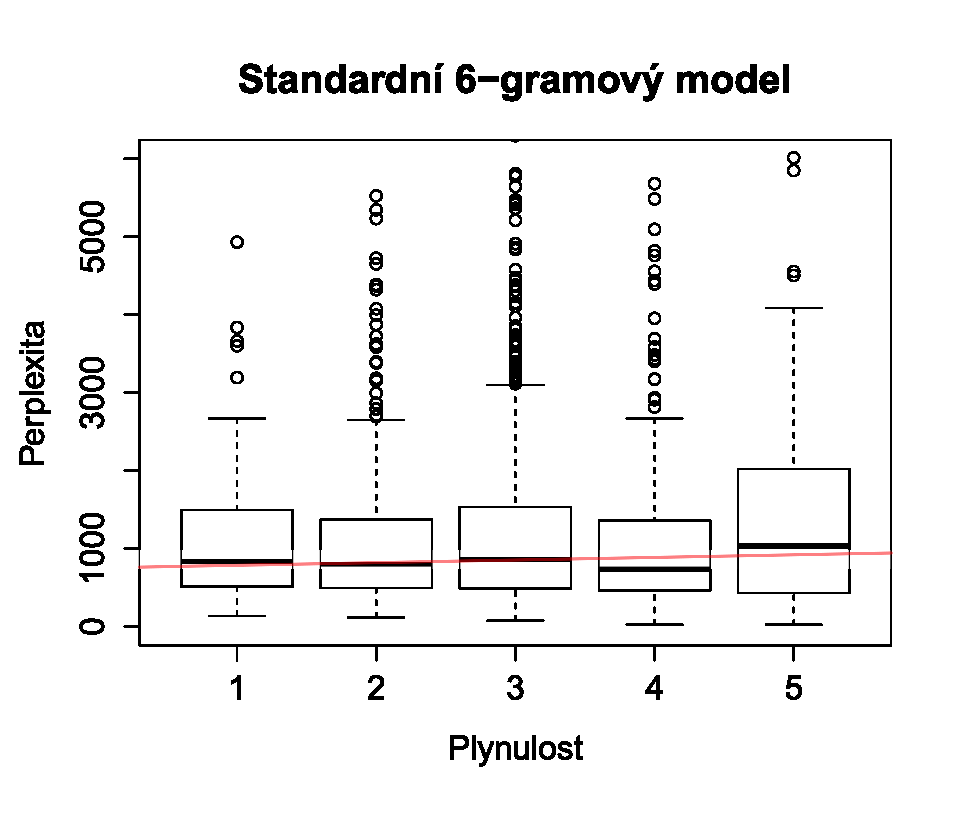
\includegraphics[width=60mm]{./grafy/morf/ngram/text.svg.eps}
	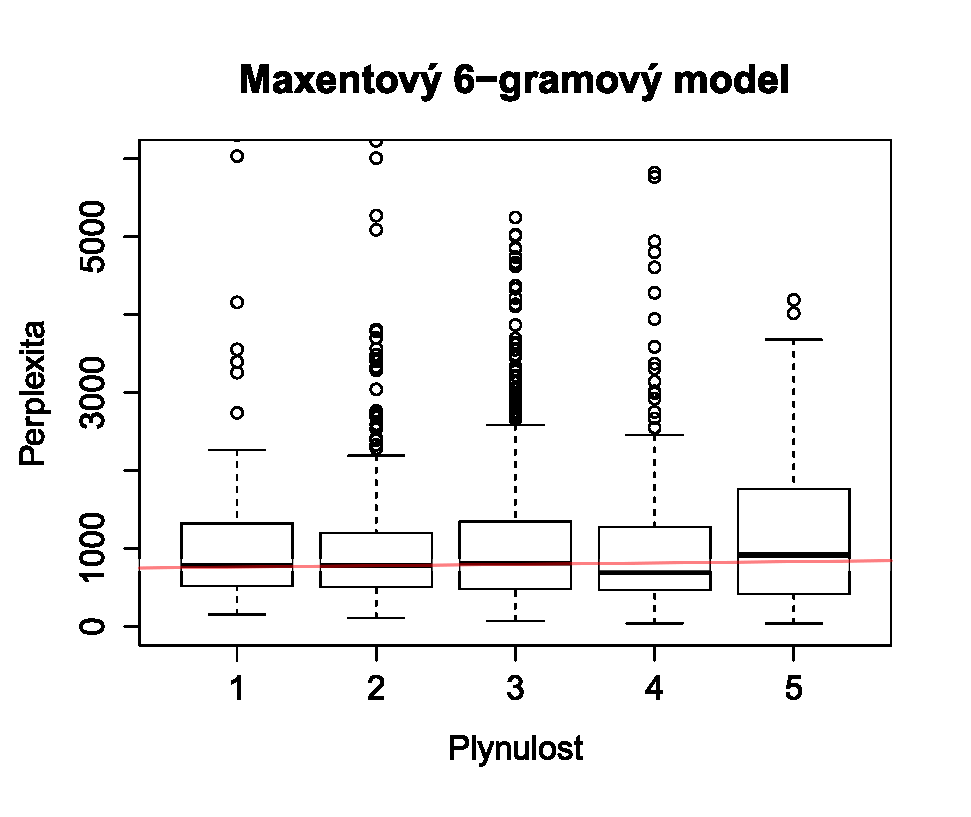
\includegraphics[width=60mm]{./grafy/morf/maxent/text.svg.eps}
\end{center}
Z obou grafů je patrné, že plynulost nekoreluje s perplexitou tak, jak jsme předpokládali. Perplexita by měla se zvyšující se plynulostí klesat - čím nižší perplexita, tím lepší a tedy i plynulejší překlad. Na obou grafech však boxploty neklesají, nýbrž kolísají. Dokonce hypotézy hodnocené plynulostí 5 mají rozsah nejčastějších perplexit nejvyšší. To ale může být částečně způsobeno malým počtem hypotéz ohodnocených plynulostí 5.
\begin{center}
	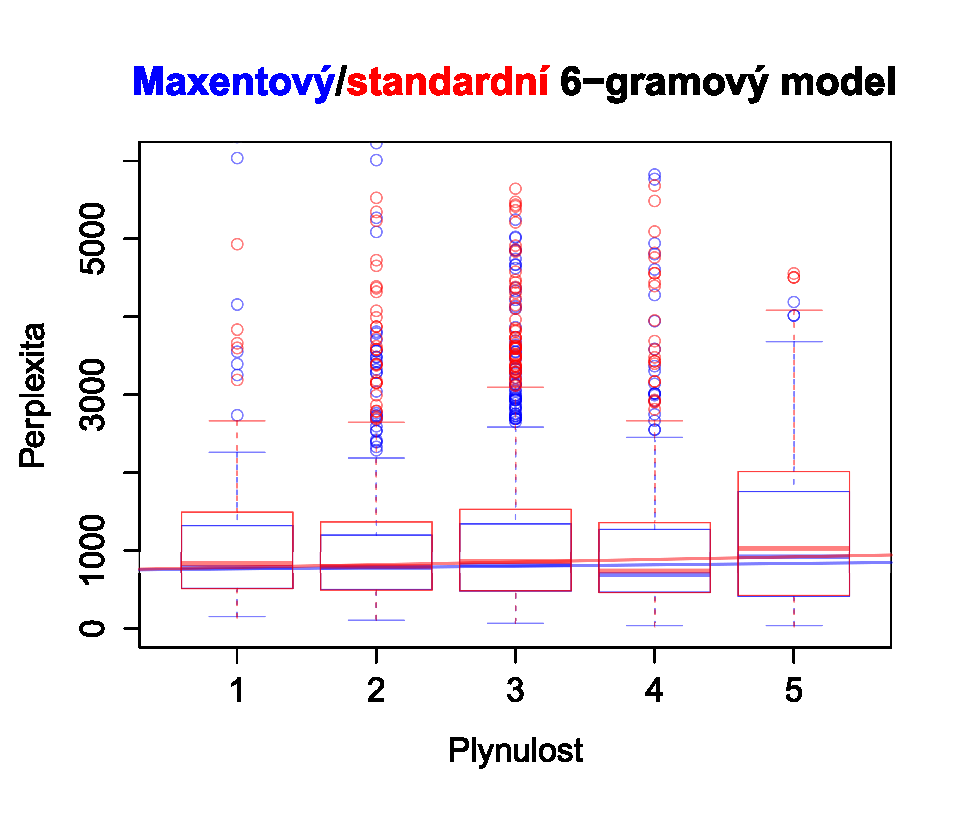
\includegraphics[width=90mm]{./grafy/morf/porovnani/text.svg.eps}
\end{center}
Srovnání ukazuje, že maxentový model dopadl o něco lépe, neboť jednotlivé boxploty mají nižší horní hranici nejčastějších perplexit než v případě standardních modelů. Rozdíly ve spodních hranicích jsou zanedbatelné.

Čas nutný k natrénování se však výrazně liší - natrénování standardního n-gramového trvalo zhruba 3 minuty oproti téměř 12 hodinám u modelu maxentového.


\section{Princip experimentů}
Německá gramatika je díky shodě jmen, pořádku slov a tvorbě větného rámce složitá. Běžné n-gramové modely, které sledují jen posloupnosti po sobě jdoucích slov nezachycují gramatiku jako takovou. Vyzkoušíme proto, zda dopadnou lépe modely, které budeme trénovat a testovat na datech, v nichž nahradíme slova za morfologické značky.

Pro morfologickou analýzu použijeme parser ParZu\footnote{The Zurich Dependency Parser for German}. Jedná se o nástroj, který kombinuje tagger Tree-Tagger a morfologický analyzátor Morphisto. ParZu za pomocí těchto dvou nástrojů vybere ze všech variant, které nabízejí, jedinou z nich a vrátí navíc větný rozbor.

připsat, že se používá předkompilovaný model morphista morphisto-02022011.a

ParZu spouští nejprve vlastní tokenizér. Vzhledem k tomu, že data z WMT 06, které používáme, jsou již tokenizovaná, tento tokenizér vynecháme a pouze upravíme formát - jeden token na řádku, věty oddělené prázdným řádkem.

Příklad výstupu ParZu:
\begin{center}
\texttt{%
\begin{tabular}{lllllllllllll}
\hline
1 & Der & der & ART & ART & Def\textbar Masc\textbar Nom\textbar Sg & 3 & det & \_ & \_ \\
2 & schönste & schön & ADJA & ADJA & Sup\textbar Masc\textbar Nom\textbar Sg\textbar Sw\textbar  & 3 & attr & \_ & \_ \\
3 & Satz & Satz & N & NN & Masc\textbar \_\textbar Sg & 0 & root & \_ & \_ \\
4 & auf & auf & PREP & APPR & \_ & 3 & pp & \_ & \_ \\
5 & aller & aller & ART & PIAT & Fem\textbar \_\textbar Sg & 6 & det & \_ & \_ \\
6 & Welt & Welt & N & NN & Fem\textbar \_\textbar Sg & 4 & pn & \_ & \_ \\
7 & . & . & \$. & \$. & \_ & 0 & root & \_ & \_ \\
\hline
\end{tabular}
}
\end{center} 

Pro účely následujících experimentů nás bude zajímat pátý a šestý sloupec - rozšířený slovní druh a morfologická analýza.

\section{Rozšířený slovní druh + morfologické značky}
Jako první zkusíme natrénovat model, kde slova nahradíme rozšířeným slovním druhem a všemi morfologickými značkami z výstupu ParZu. Pro oddělení použijeme dvojtečku.


Příklad věty:
\begin{center}
\texttt{%
\arrayrulecolor{seda}
\begin{tabular}{llll}
\color{red} Die & \color{red} unabhängige & \color{red} Justiz\\
\color{blue} ART:Def\textbar Fem\textbar Akk\textbar Sg & \color{blue} ADJA:Pos\textbar Fem\textbar Akk\textbar Sg\textbar \_\textbar & \color{blue} NN:Fem\textbar Akk\textbar Sg \\
\hline
\color{black}
\color{red} und & \color{red} die & \color{red} freien \\
\color{blue} KON:\_ & \color{blue} ART:Def\textbar Neut\textbar Akk\textbar Pl & \color{blue} ADJA:Pos\textbar Neut\textbar Akk\textbar Pl\textbar \_\textbar \\
\hline
\color{red} Medien & \color{red} zu & \color{red} unterdrücken & \color{red} . \\
\color{blue} NN:Neut\textbar Akk\textbar Pl & \color{blue} PTKZU:\_ & \color{blue} VVINF:\_ & \color{blue} \$.:\_ \\
\hline
\end{tabular}
}
\end{center}

\begin{center}		
	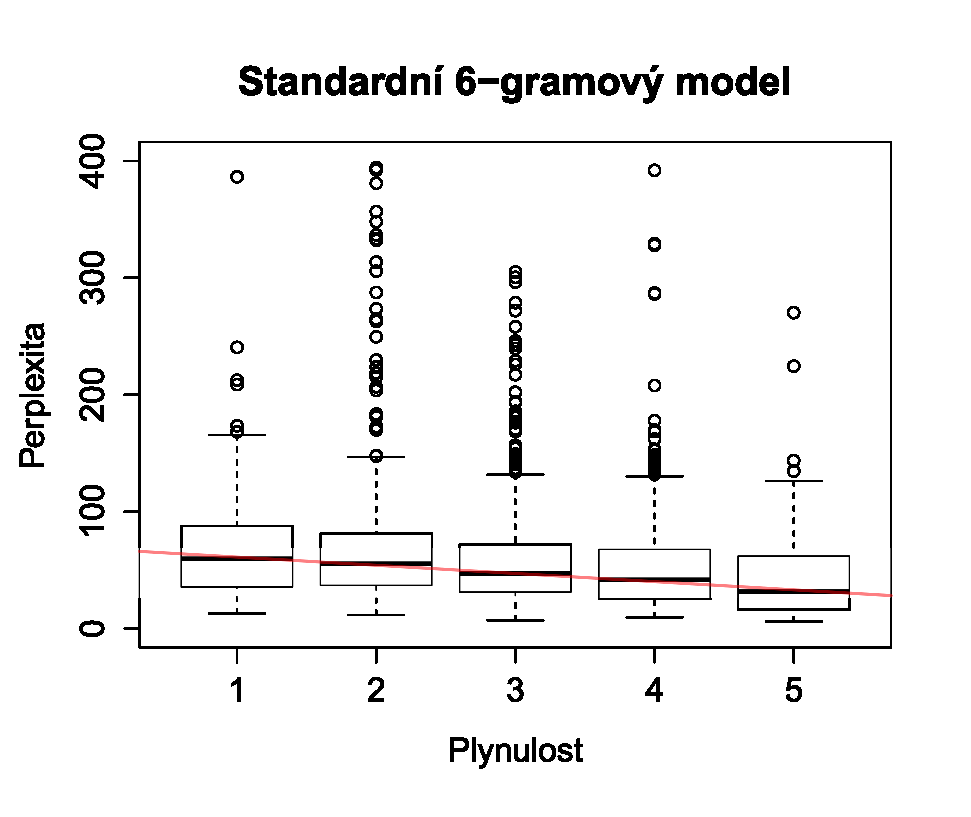
\includegraphics[width=60mm]{./grafy/morf/ngram/all.svg.eps}	
	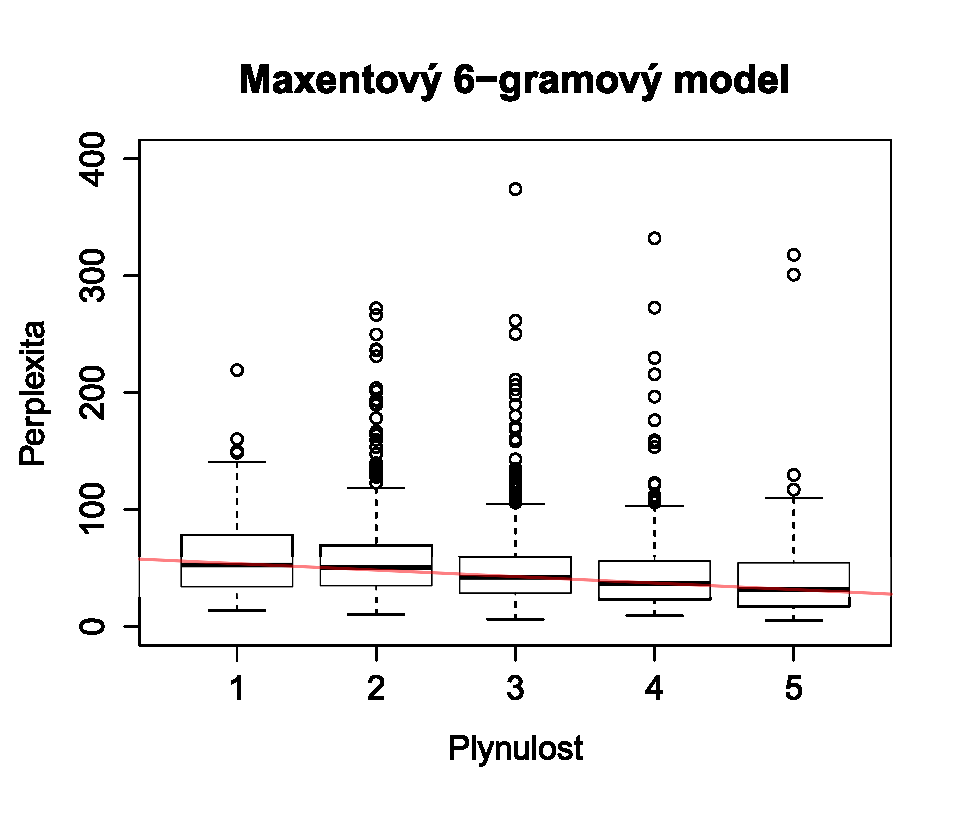
\includegraphics[width=60mm]{./grafy/morf/maxent/all.svg.eps}	
\end{center}

\begin{center}	
	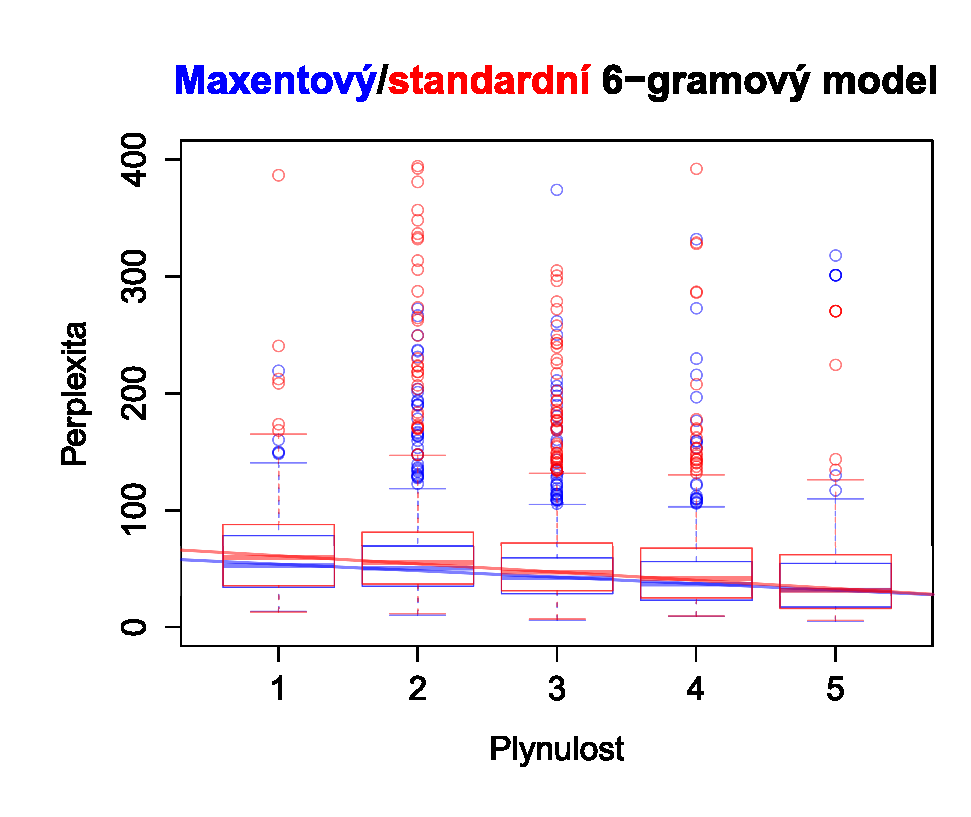
\includegraphics[width=90mm]{./grafy/morf/porovnani/all.svg.eps}	
\end{center}
Maxentové modely opět dopadají lépe než standardní n-gramové. Celkově dopadly všechny modely lépe než běžné modely se slovy, neboť zde mají boxploty už klesavou tendenci.

Z hlediska výpočetních nároků TABULKA?

Tyto modely sice obsahují morfologickou analýzu, ale nerozumí gramatice jako takové. Nedokáží rozlišit, zda se sousední jména shodují v rodě, ale už ne v pádě apod. Natrénování maxentového modelu s rysy, které by vycházely z morfologické analýzy (rod, pád, číslo, ...), rozšíření SRILMu od Tanela Alumäe, jež používáme, bohužel neumožňuje a jiné dostupné toolkity, např. Maxent toolkit od LeZhanga, nejsou vhodné z hlediska výpočetních nároků na velká data. Zkusíme proto natrénovat další modely, ve kterých nahradíme slova vždy jedním z potencionálních rysů. 

\section{Rozšířený slovní druh}
\begin{center}
	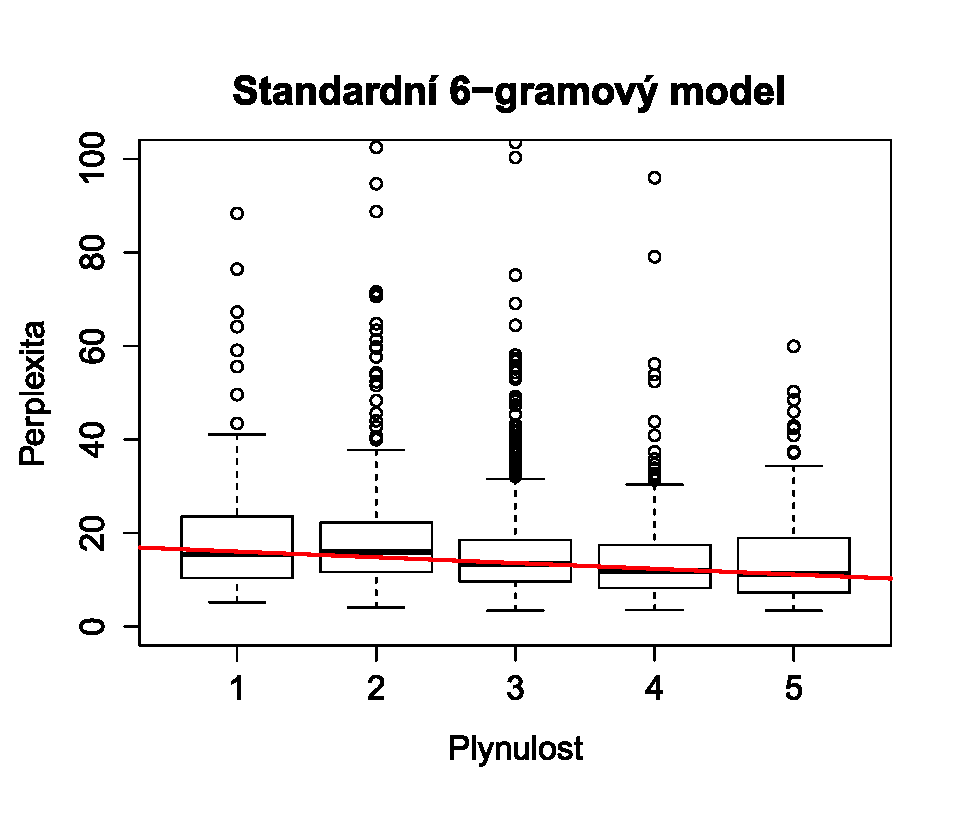
\includegraphics[width=60mm]{./grafy/morf/ngram/rsd.svg.eps}
	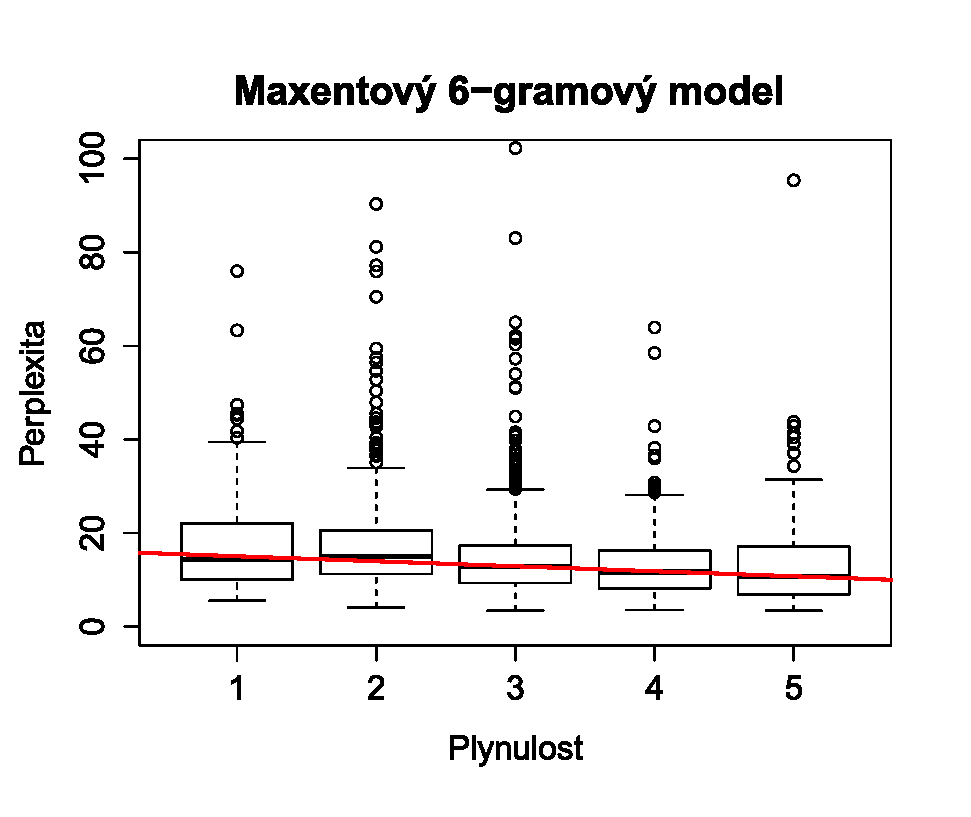
\includegraphics[width=60mm]{./grafy/morf/maxent/rsd.svg.eps}
	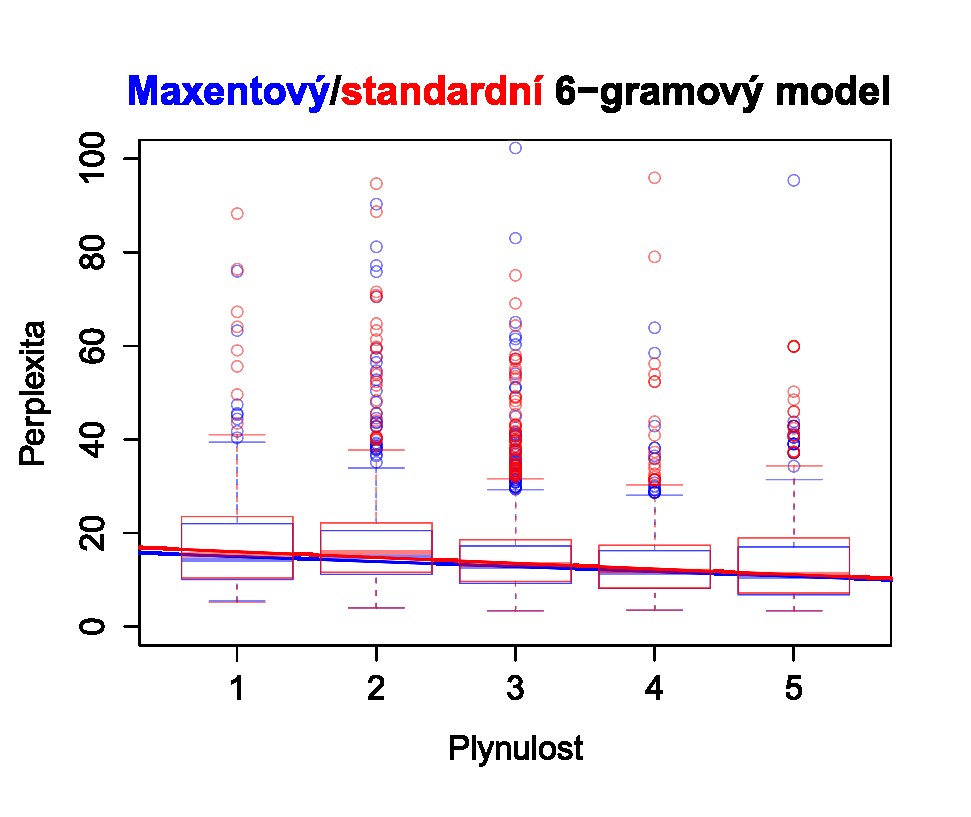
\includegraphics[width=90mm]{./grafy/morf/porovnani/rsd.svg.eps}	
\end{center}

\section{Rod}
První z modelů s jednou morfologickou značkou budou modely obsahující rod. Slova budou nahrazena znakem \texttt{w}, ke kterému se připojí patřičný rod, lze-li u slova určit.

Příklad věty:
\begin{center}
\texttt{%
\arrayrulecolor{seda}
\begin{tabular}{lllllll}
\color{red} Die & \color{red} unabhängige & \color{red} Justiz & \color{red} und & \color{red} die & \color{red} freien & \color{red} Medien\\
\color{blue} wFem & \color{blue} wFem & \color{blue} wFem & \color{blue} w & \color{blue} wNeut & \color{blue} wNeut & \color{blue} wNeut\\
\hline
\color{red} zu & \color{red} unterdrücken &\color{red} .\\
\color{blue} w & \color{blue} w & \color{blue} w \\
\hline
\end{tabular}
}
\end{center}
 

\begin{center}
	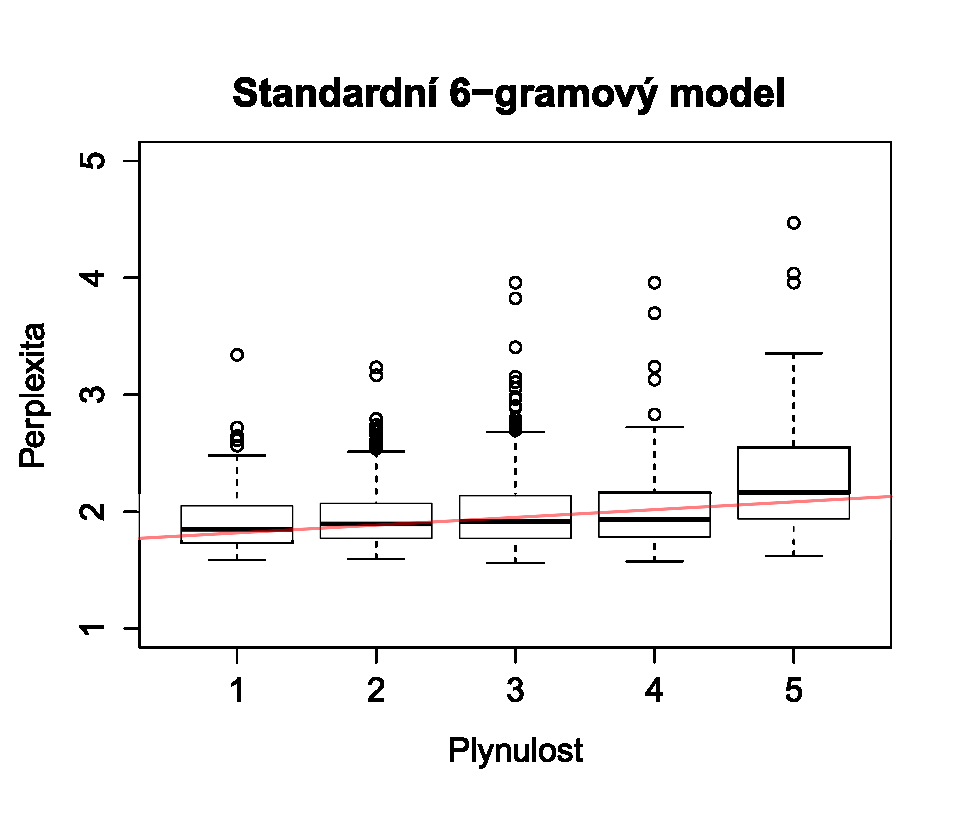
\includegraphics[width=60mm]{./grafy/morf/ngram/rod.svg.eps}
	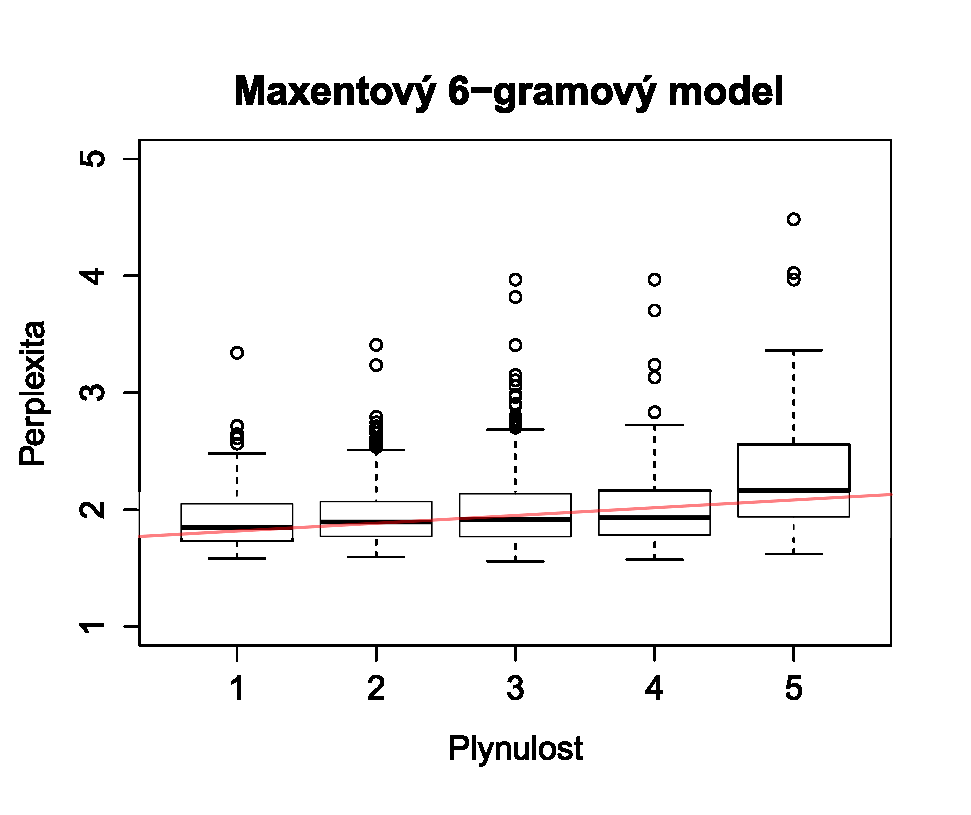
\includegraphics[width=60mm]{./grafy/morf/maxent/rod.svg.eps}
	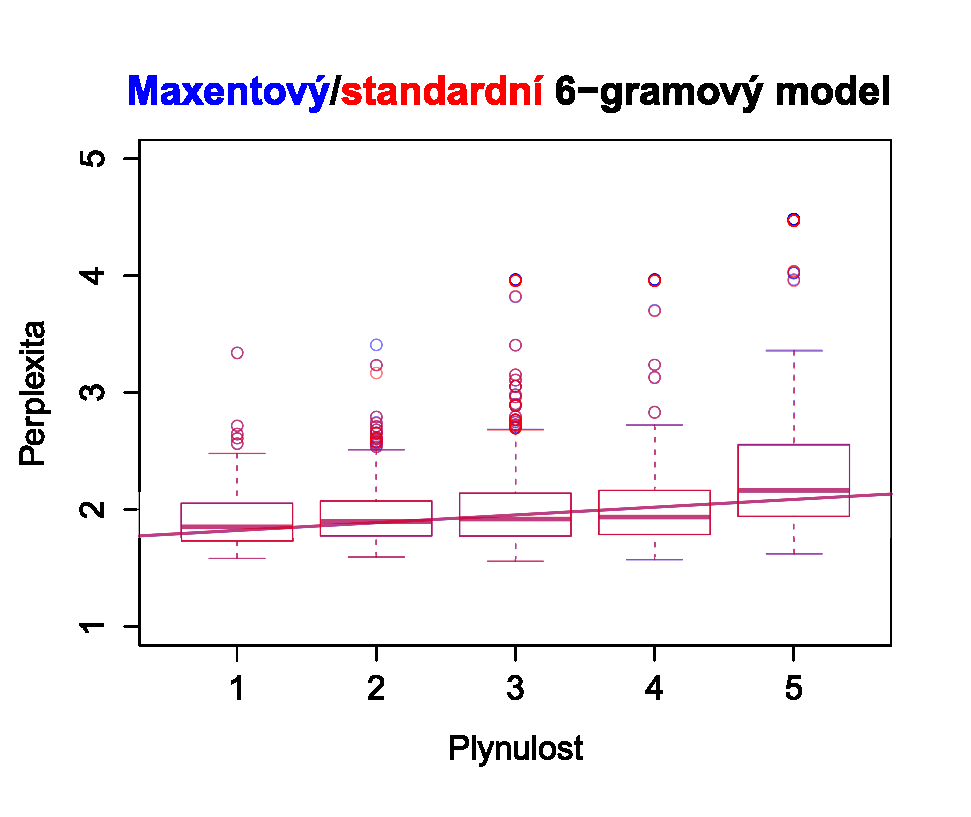
\includegraphics[width=90mm]{./grafy/morf/porovnani/rod.svg.eps}	
\end{center}
\subsection{Rod stejný s předchozím}
\begin{center}
	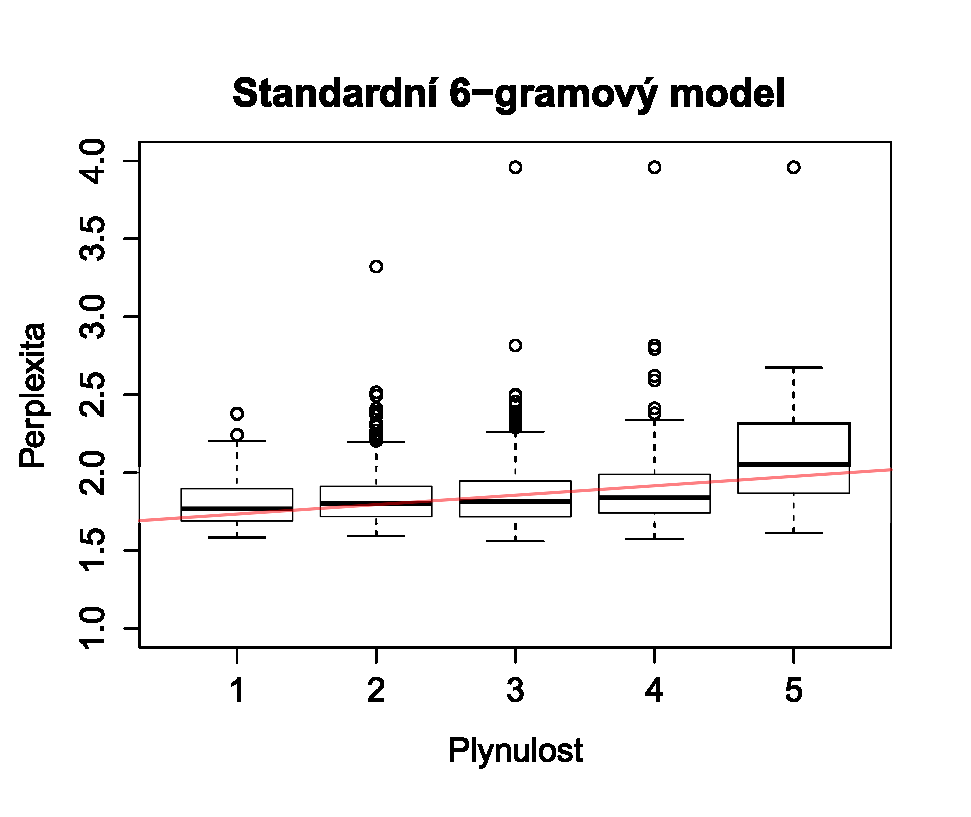
\includegraphics[width=60mm]{./grafy/morf/ngram/rodstejny.svg.eps}
	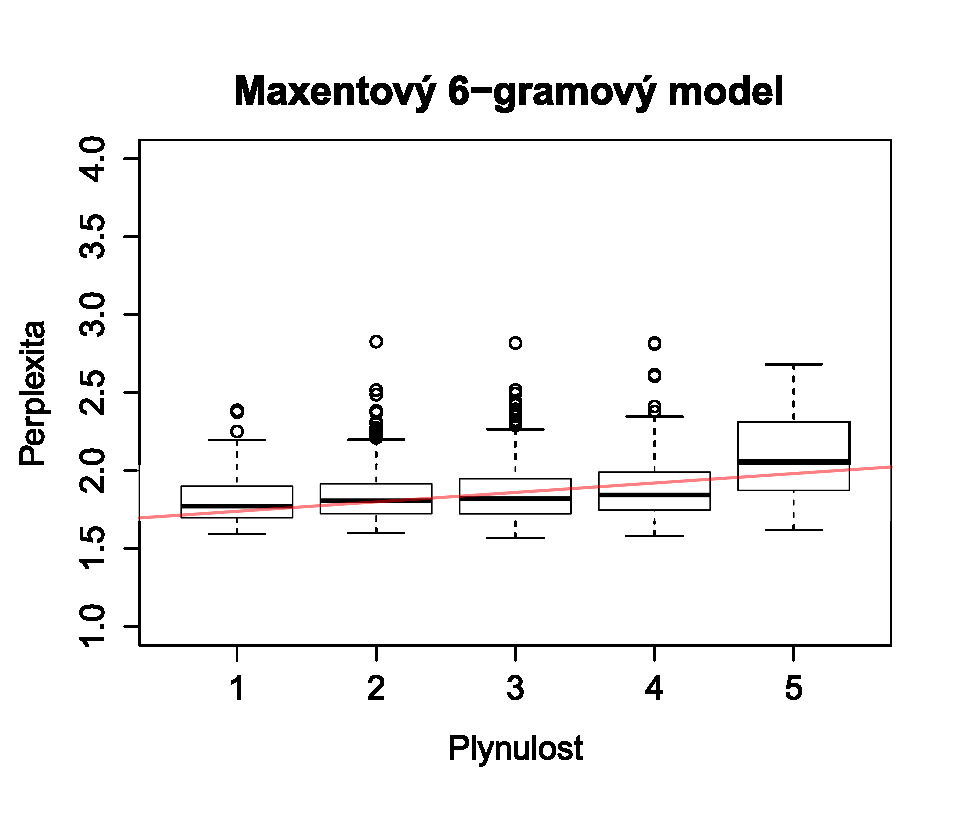
\includegraphics[width=60mm]{./grafy/morf/maxent/rodstejny.svg.eps}
	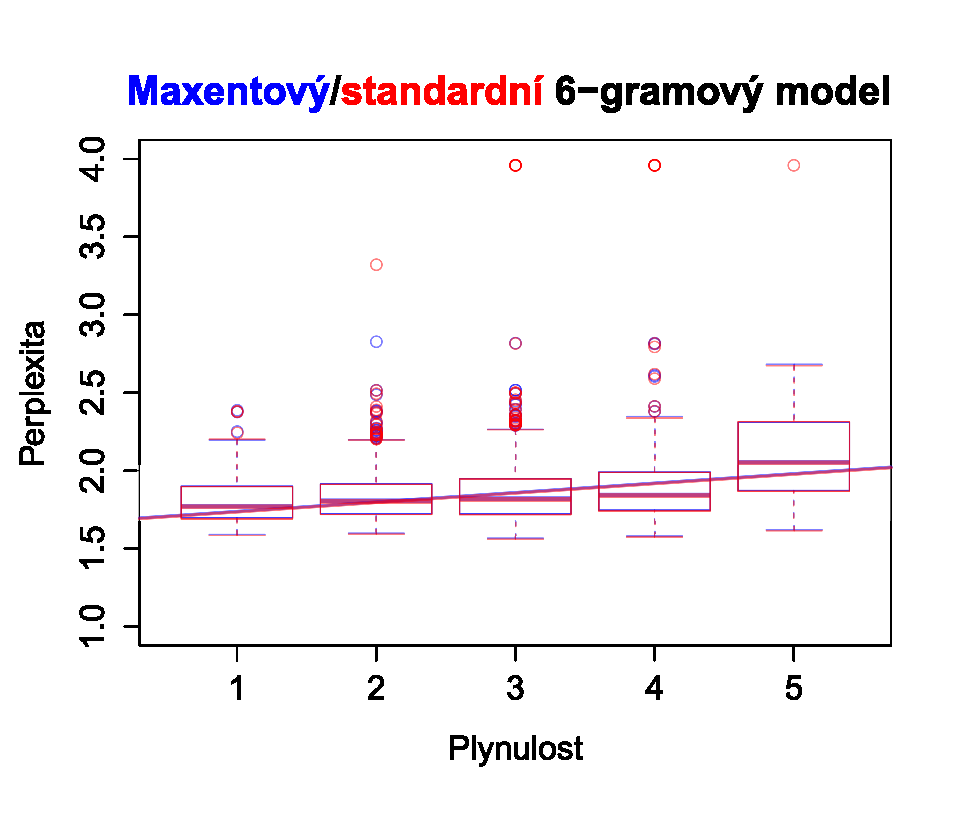
\includegraphics[width=90mm]{./grafy/morf/porovnani/rodstejny.svg.eps}	
\end{center}
\subsection{PŘIDAT RSD TAKHLE POD KAŽDÝ?}
\subsection{S rozšířeným slovním druhem}
\begin{center}
	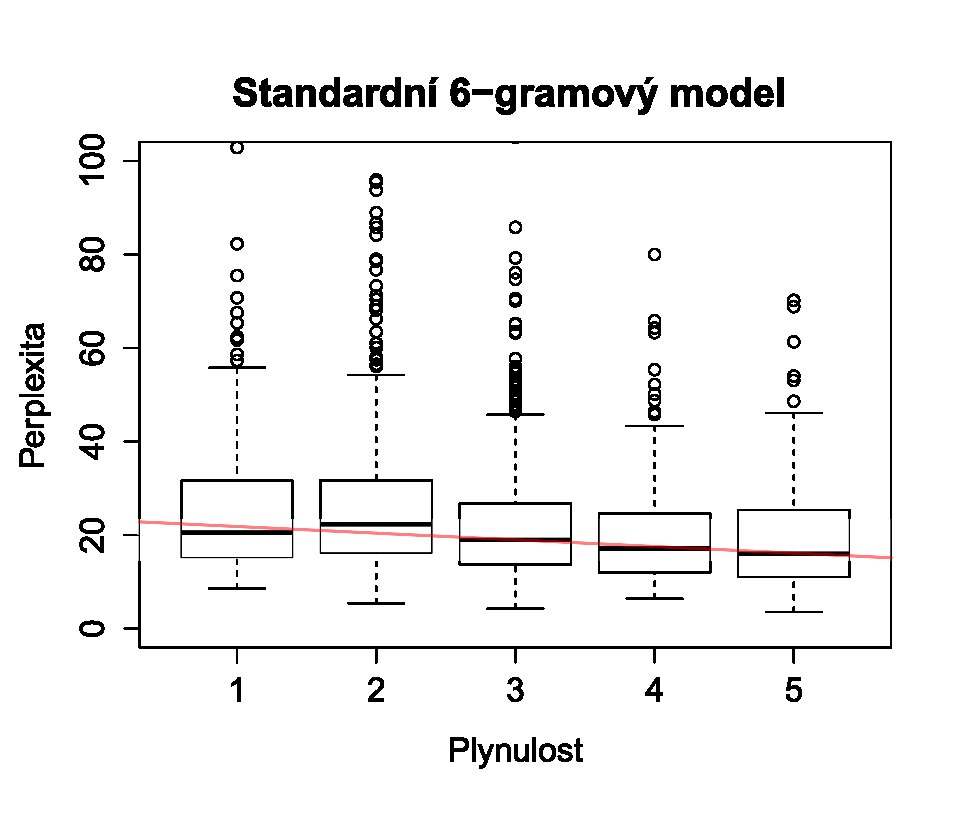
\includegraphics[width=60mm]{./grafy/morf/ngram/rsd+rod.svg.eps}
	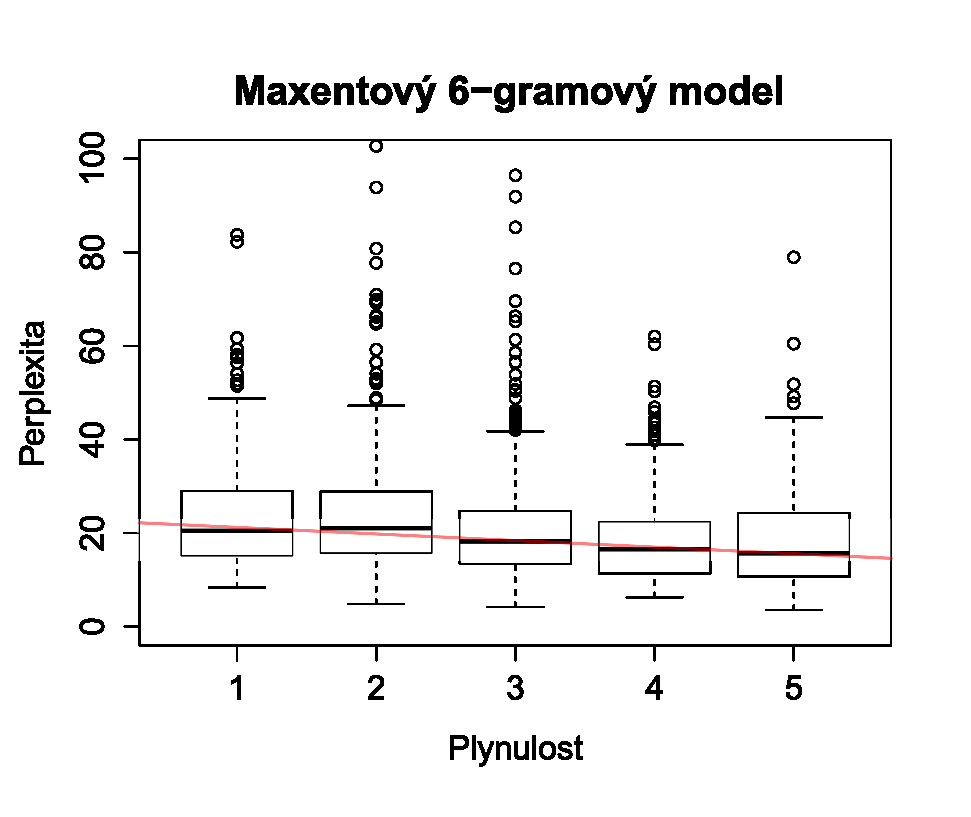
\includegraphics[width=60mm]{./grafy/morf/maxent/rsd+rod.svg.eps}
	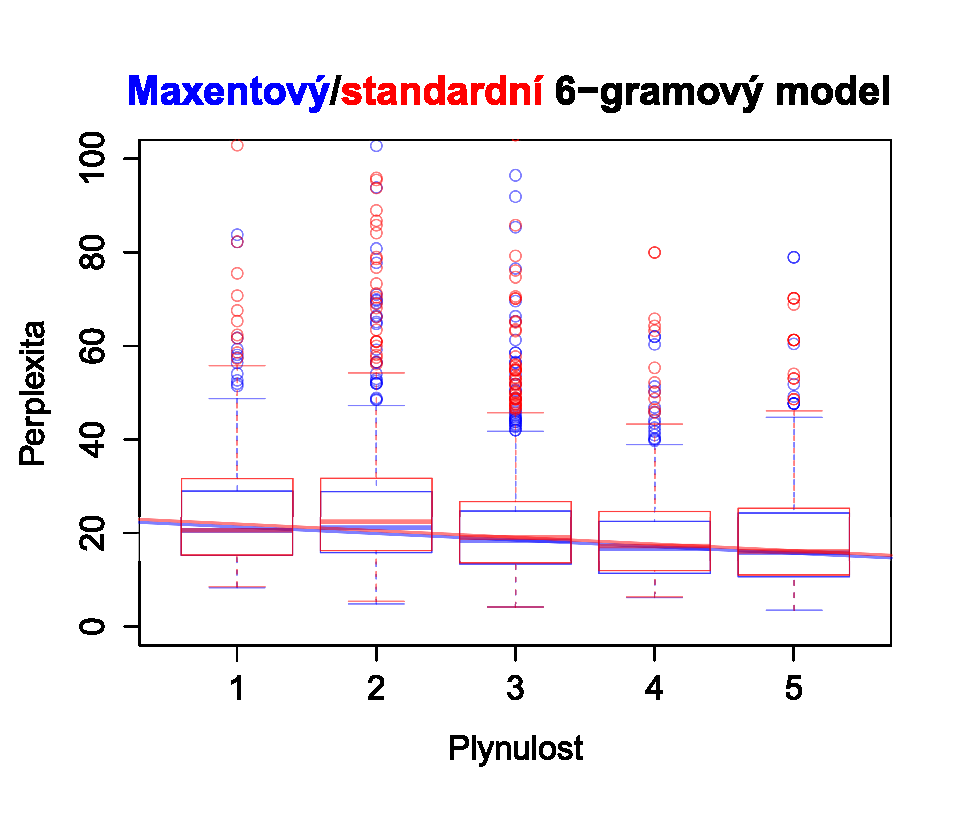
\includegraphics[width=90mm]{./grafy/morf/porovnani/rsd+rod.svg.eps}	
\end{center}

\section{Číslo}
\begin{center}
	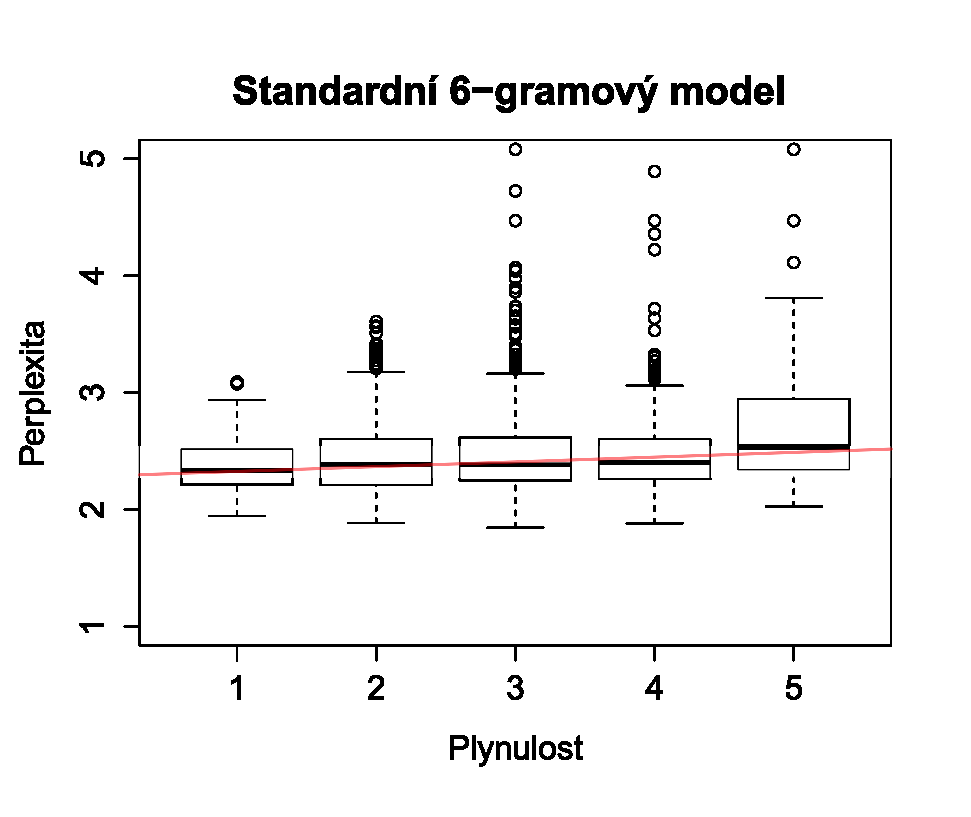
\includegraphics[width=60mm]{./grafy/morf/ngram/cislo.svg.eps}
	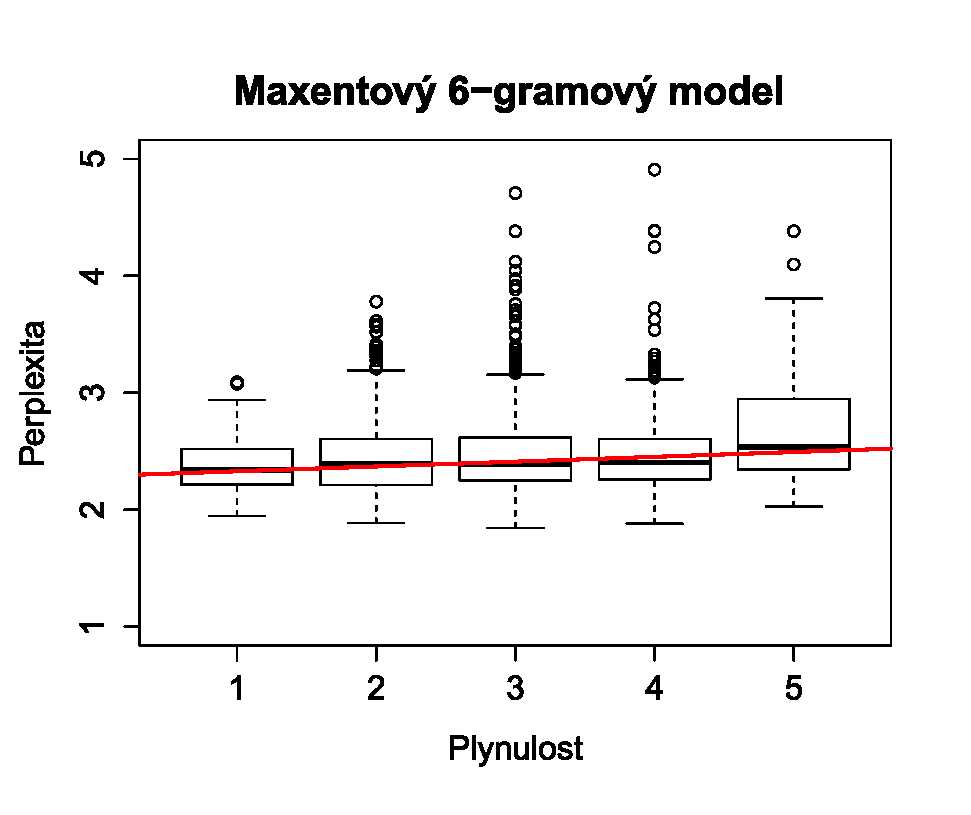
\includegraphics[width=60mm]{./grafy/morf/maxent/cislo.svg.eps}	
	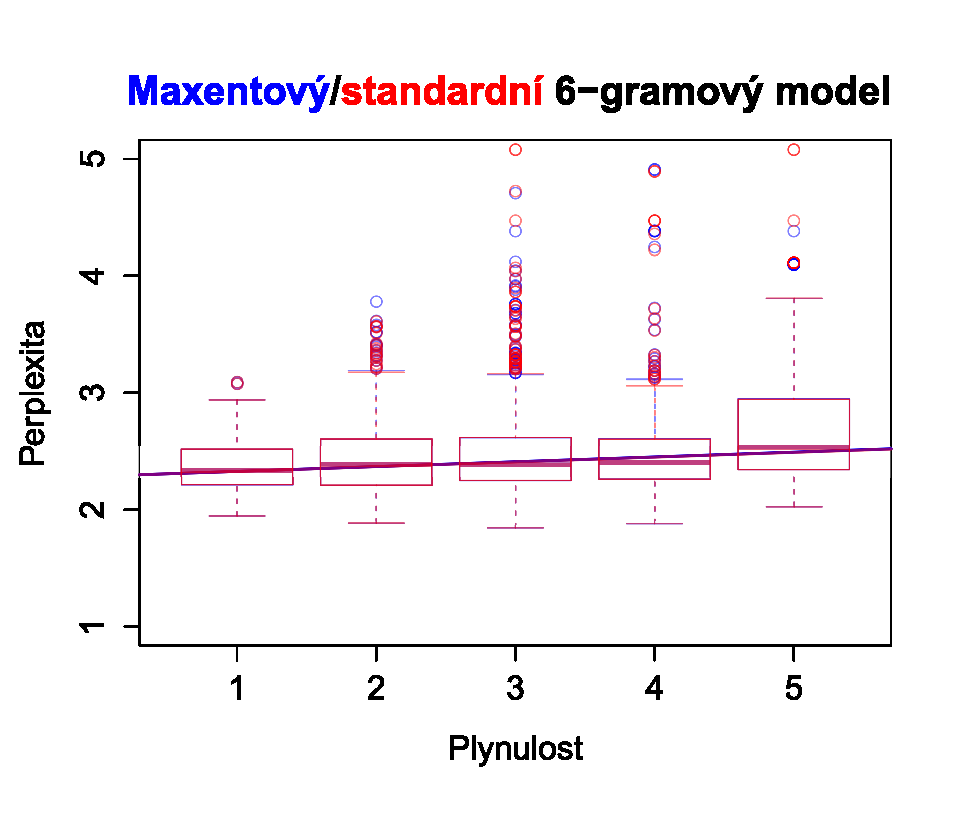
\includegraphics[width=90mm]{./grafy/morf/porovnani/cislo.svg.eps}
\end{center}
\section{Pád}
\begin{center}
	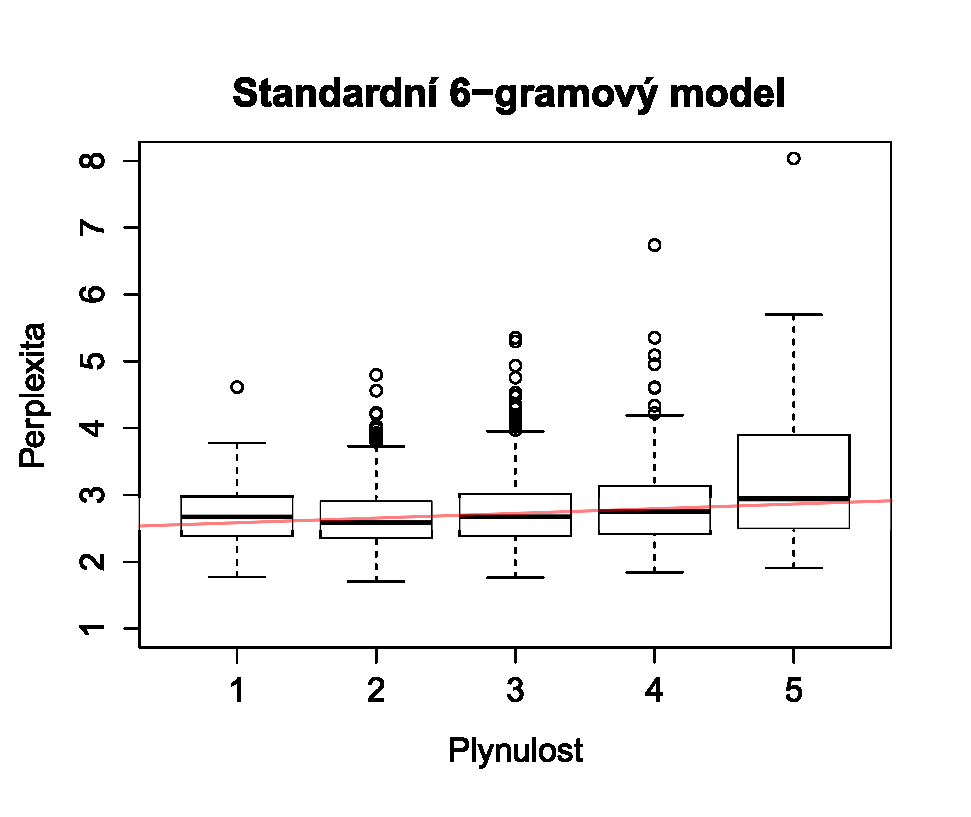
\includegraphics[width=60mm]{./grafy/morf/ngram/pad.svg.eps}
	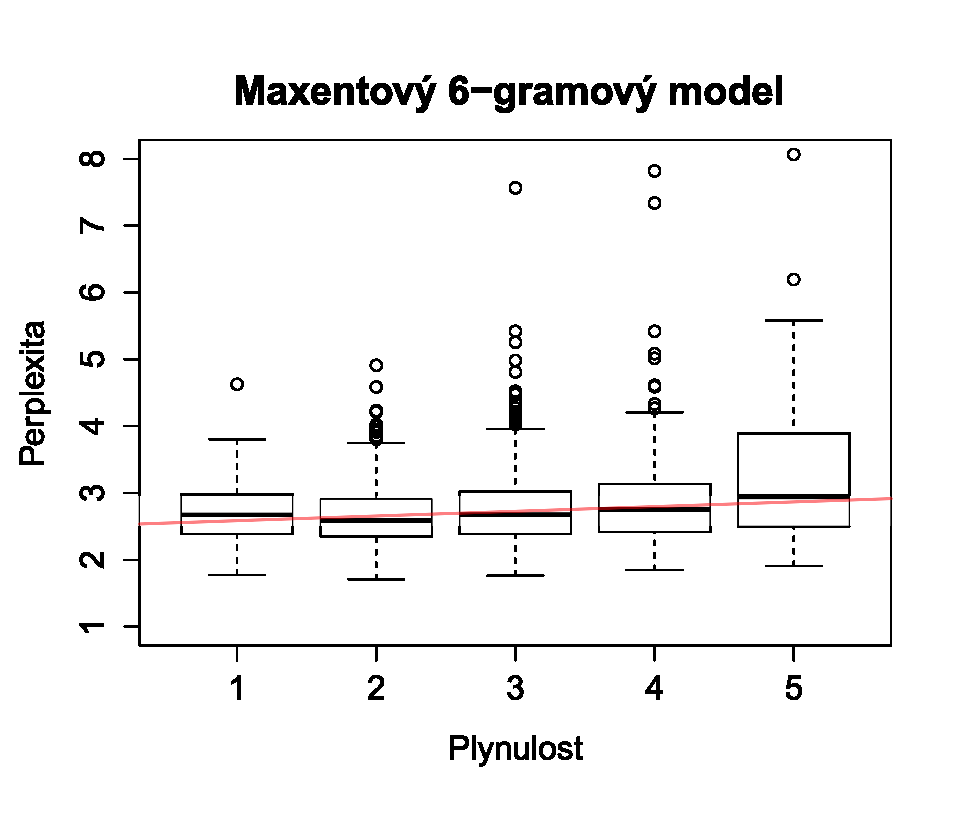
\includegraphics[width=60mm]{./grafy/morf/maxent/pad.svg.eps}	
	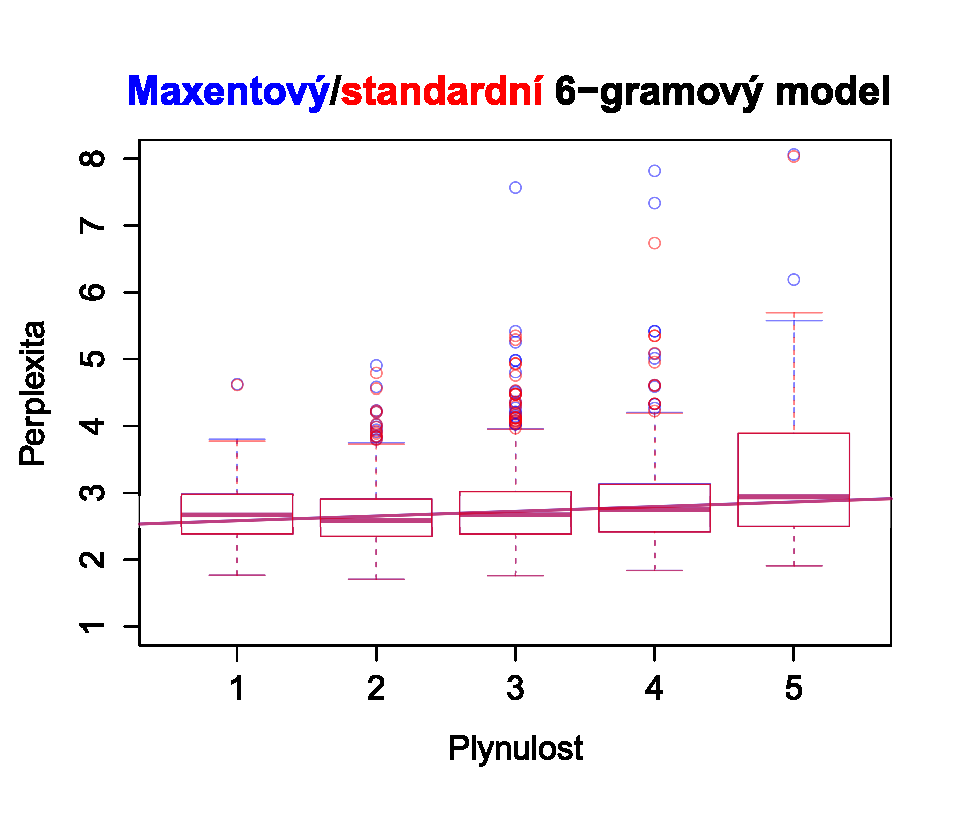
\includegraphics[width=90mm]{./grafy/morf/porovnani/pad.svg.eps}	
\end{center}

\section{Osoba + číslo}
\begin{center}
	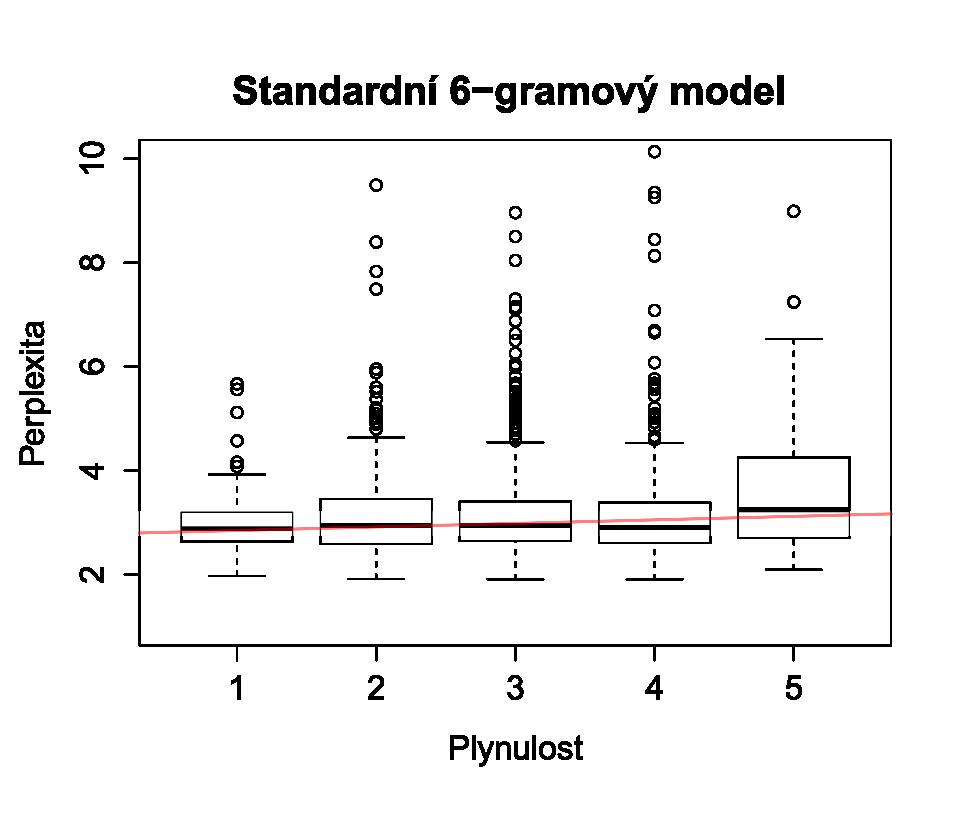
\includegraphics[width=60mm]{./grafy/morf/ngram/osoba+cislo.svg.eps}
	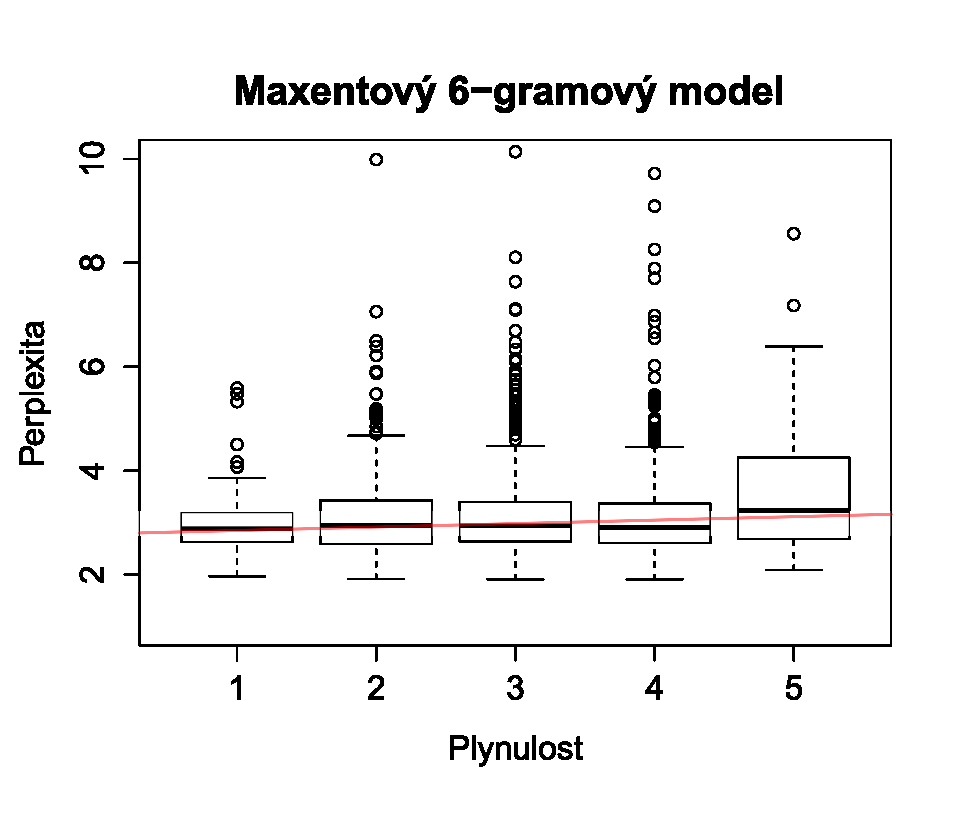
\includegraphics[width=60mm]{./grafy/morf/maxent/osoba+cislo.svg.eps}	
	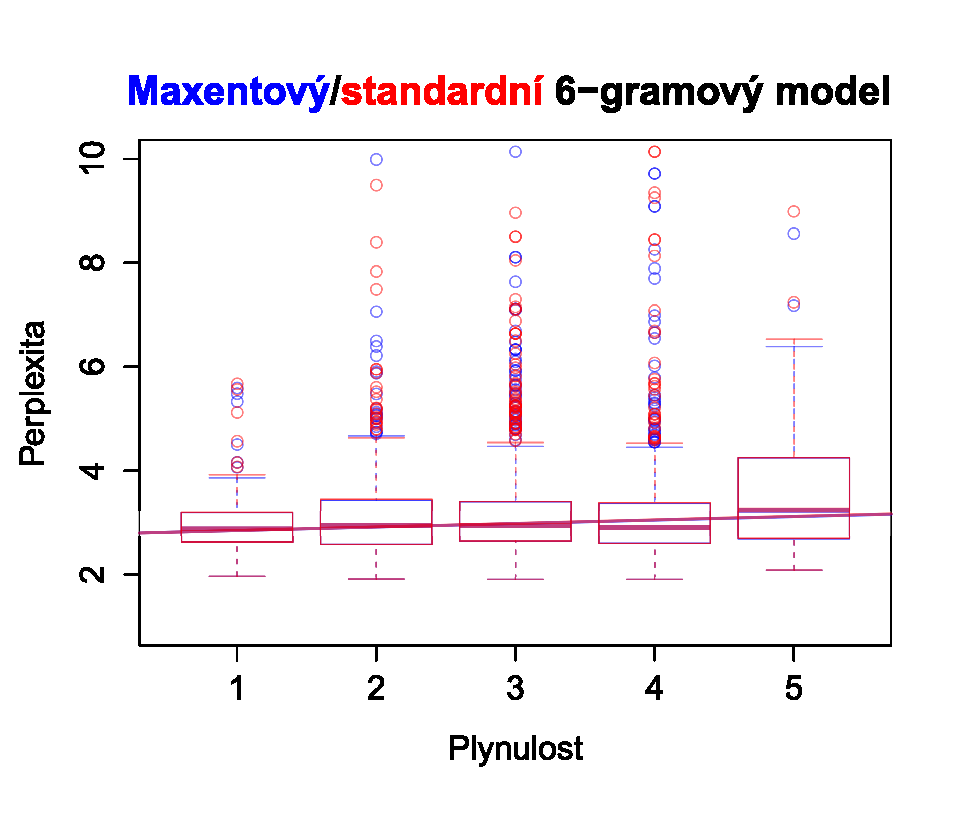
\includegraphics[width=90mm]{./grafy/morf/porovnani/osoba+cislo.svg.eps}	
\end{center}
\section{Rozšířený slovní druh + rod}
\begin{center}
	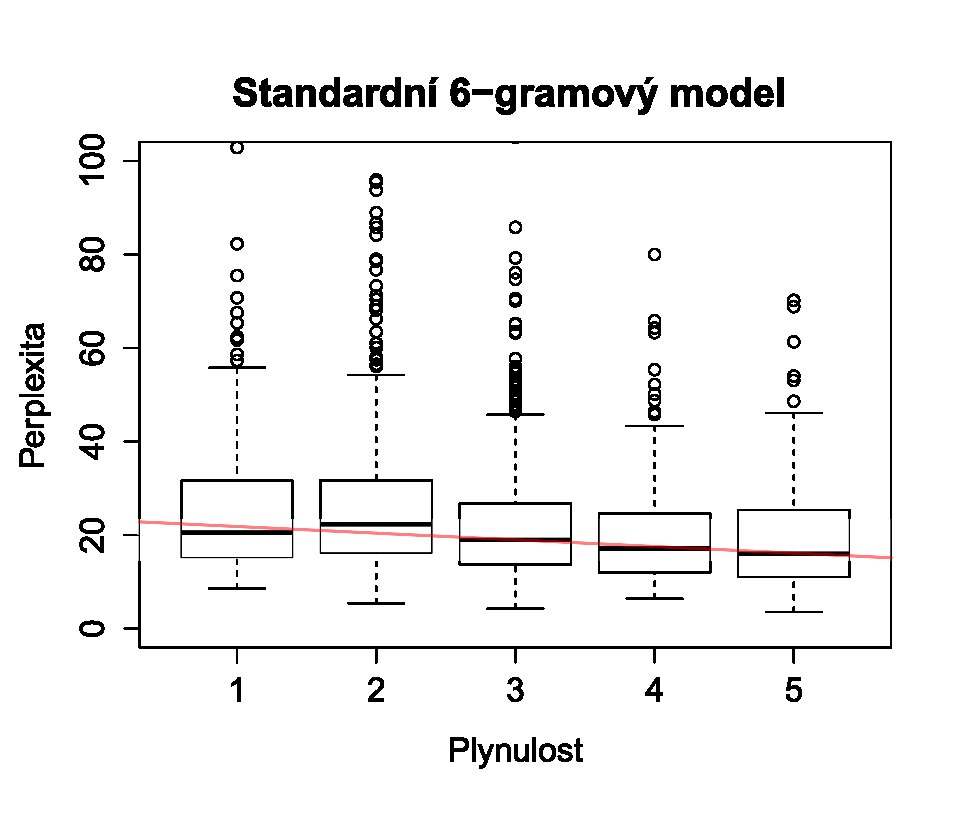
\includegraphics[width=60mm]{./grafy/morf/ngram/rsd+rod.svg.eps}
	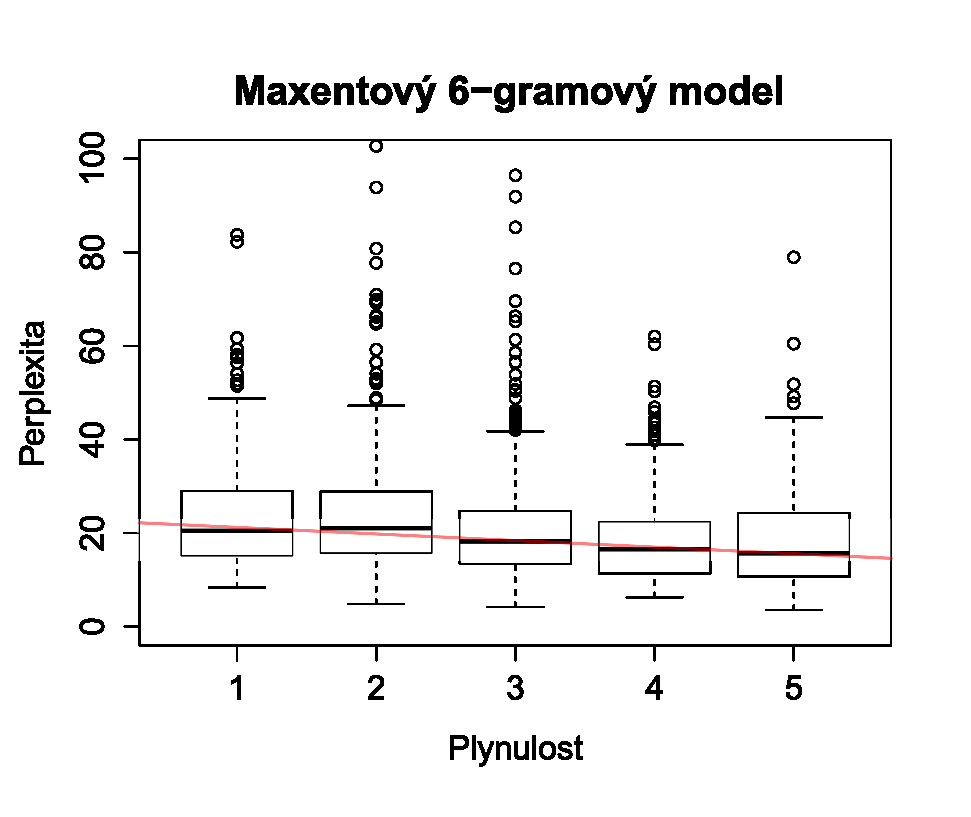
\includegraphics[width=60mm]{./grafy/morf/maxent/rsd+rod.svg.eps}
	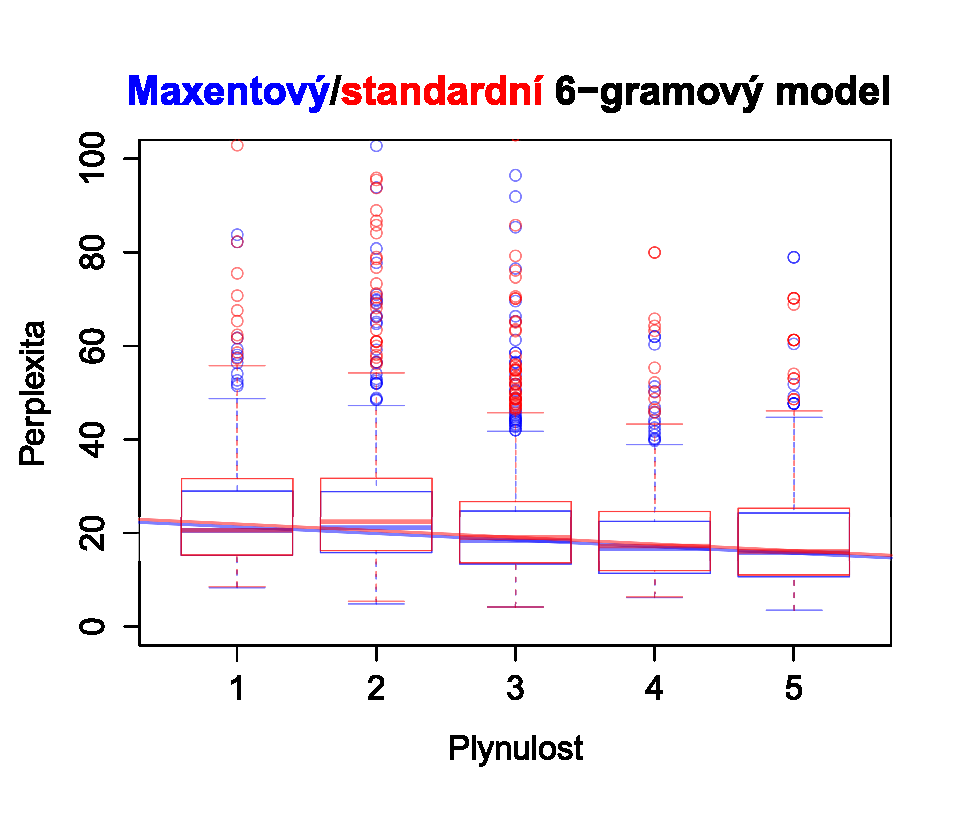
\includegraphics[width=90mm]{./grafy/morf/porovnani/rsd+rod.svg.eps}	
\end{center}
\section{Rozšířený slovní druh + pád}
\begin{center}
	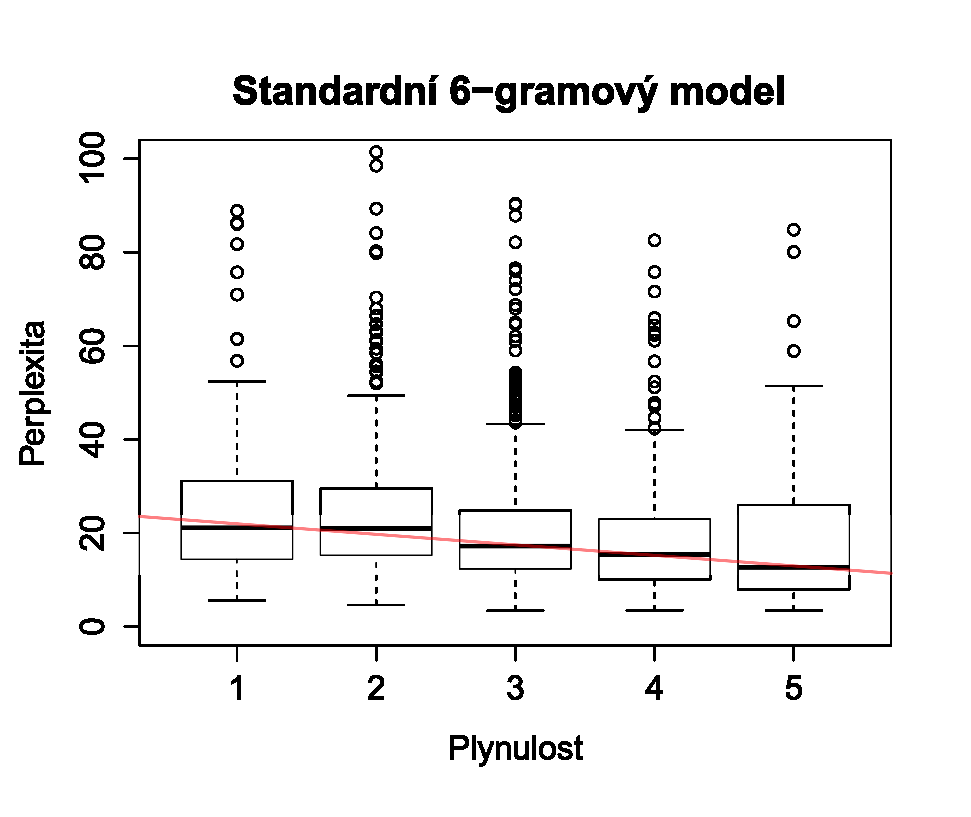
\includegraphics[width=60mm]{./grafy/morf/ngram/rsd+pad.svg.eps}
	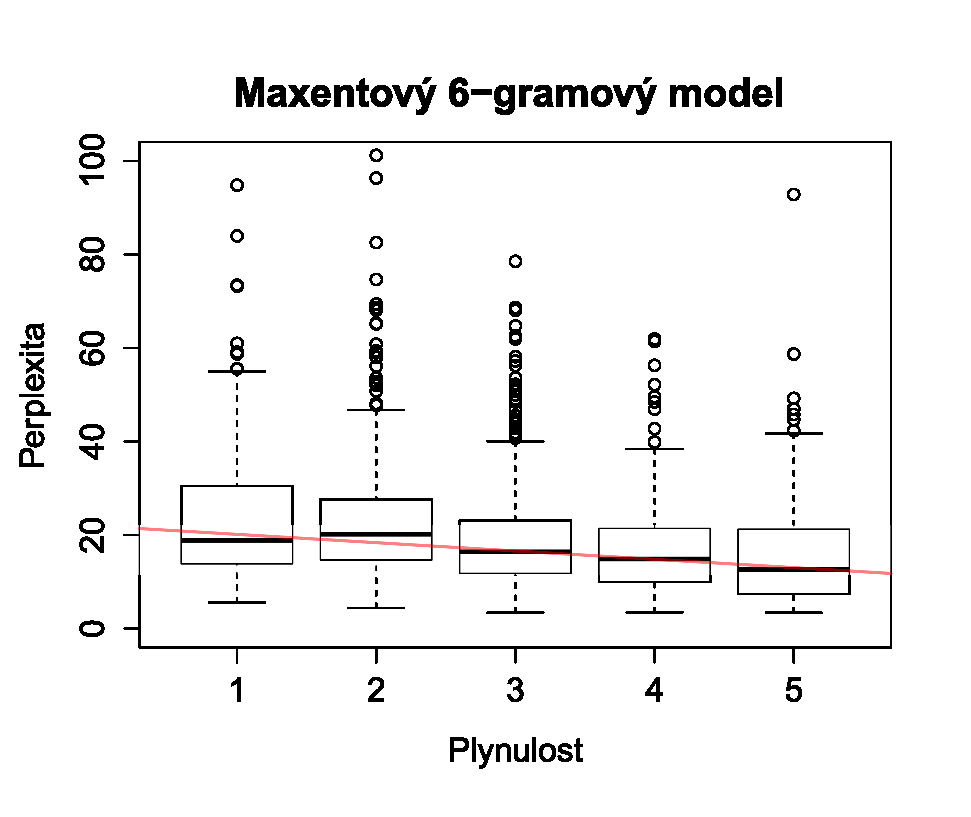
\includegraphics[width=60mm]{./grafy/morf/maxent/rsd+pad.svg.eps}
	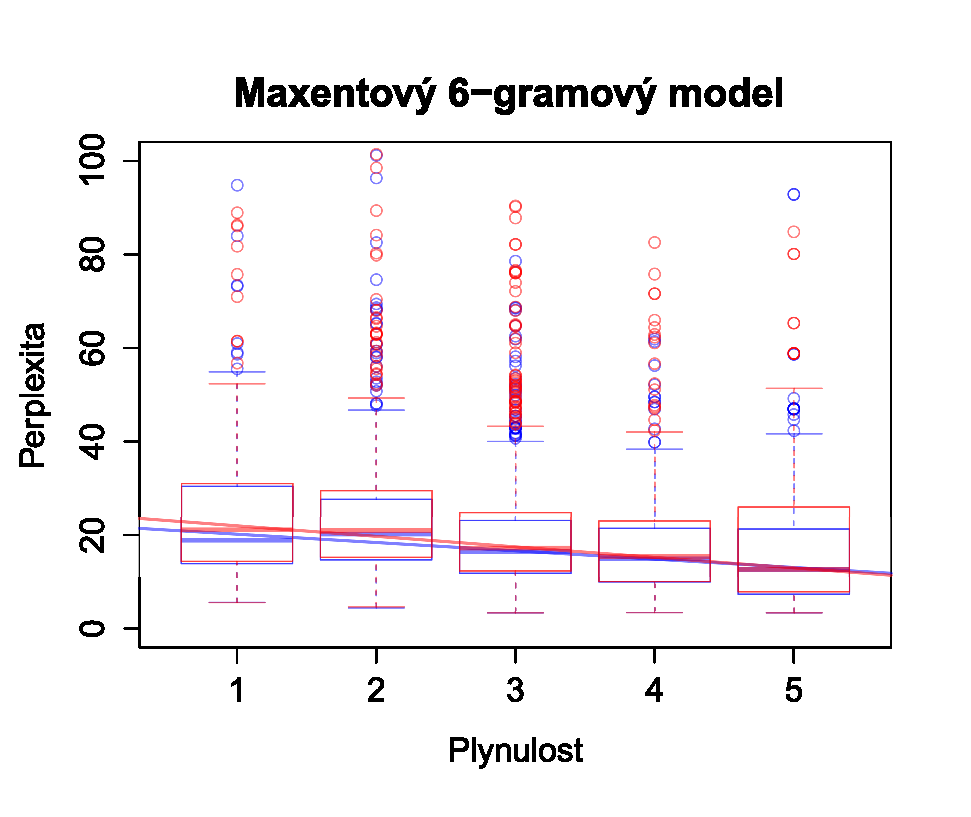
\includegraphics[width=90mm]{./grafy/morf/porovnani/rsd+pad.svg.eps}	
\end{center}
\section{Rozšířený slovní druh + číslo}
\begin{center}
	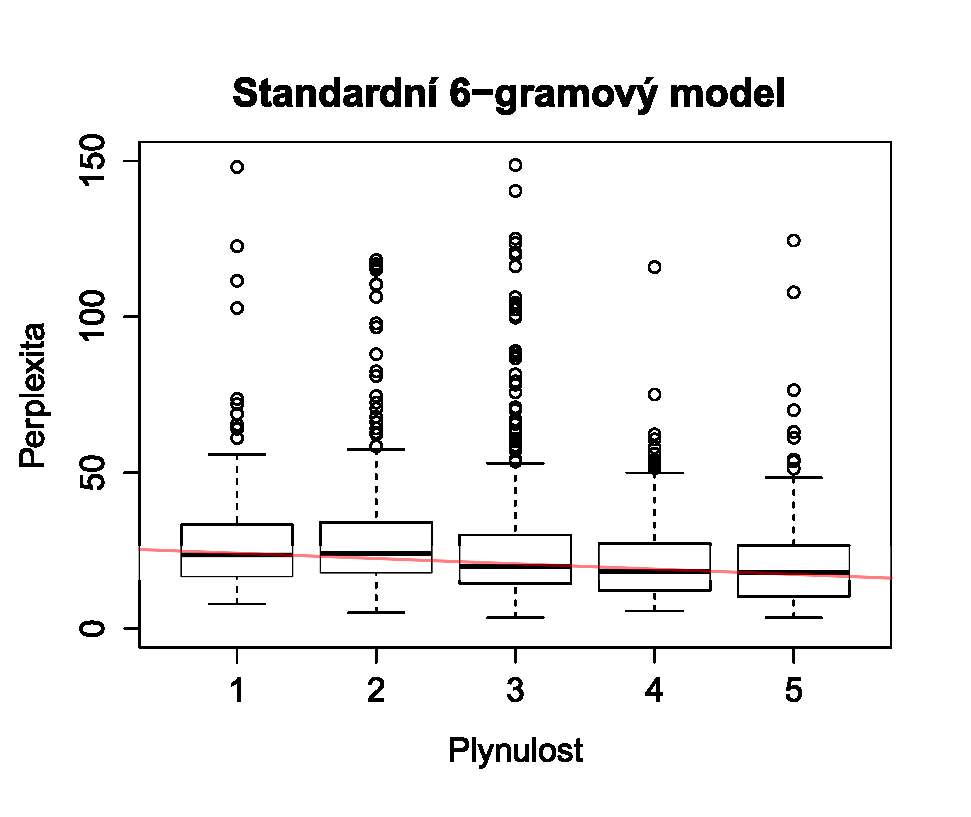
\includegraphics[width=60mm]{./grafy/morf/ngram/rsd+cislo.svg.eps}
	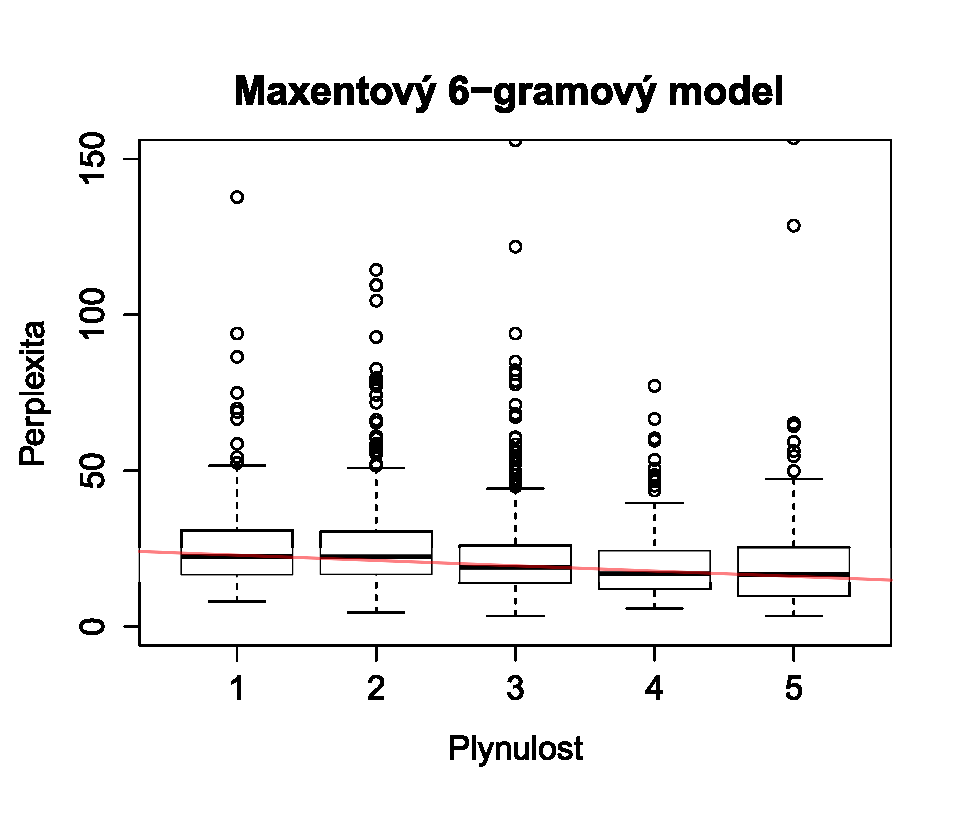
\includegraphics[width=60mm]{./grafy/morf/maxent/rsd+cislo.svg.eps}
	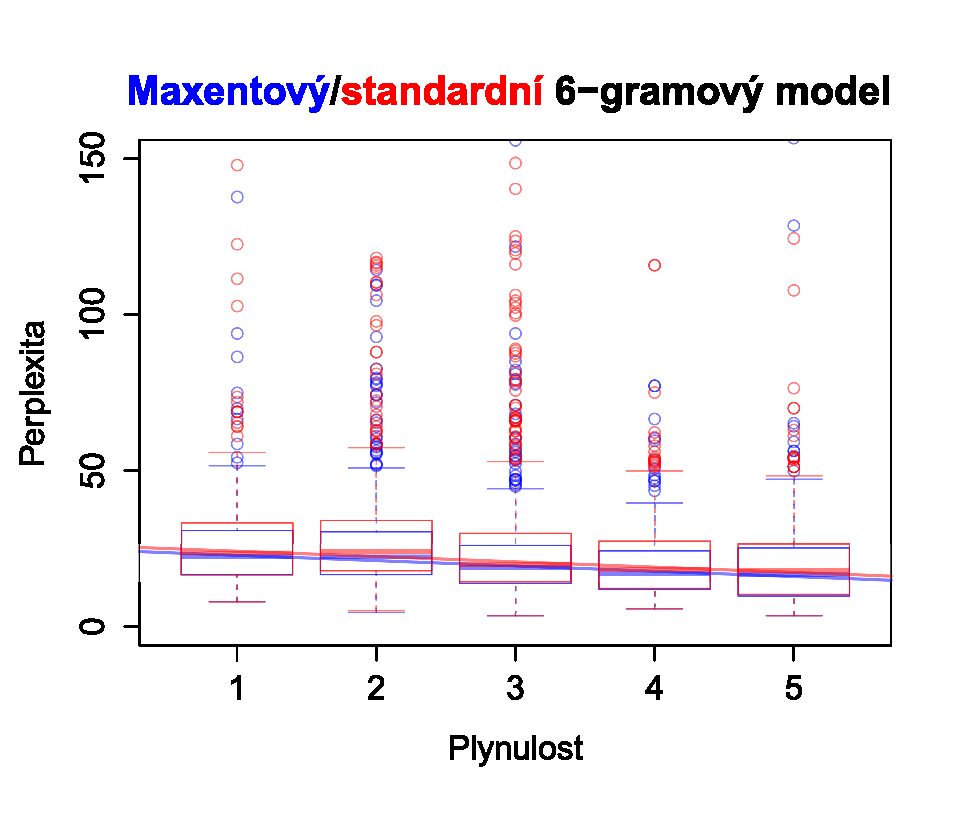
\includegraphics[width=90mm]{./grafy/morf/porovnani/rsd+cislo.svg.eps}	
\end{center}

\section{Porovnání z hlediska výpočetních nároků}
\begin{center}
	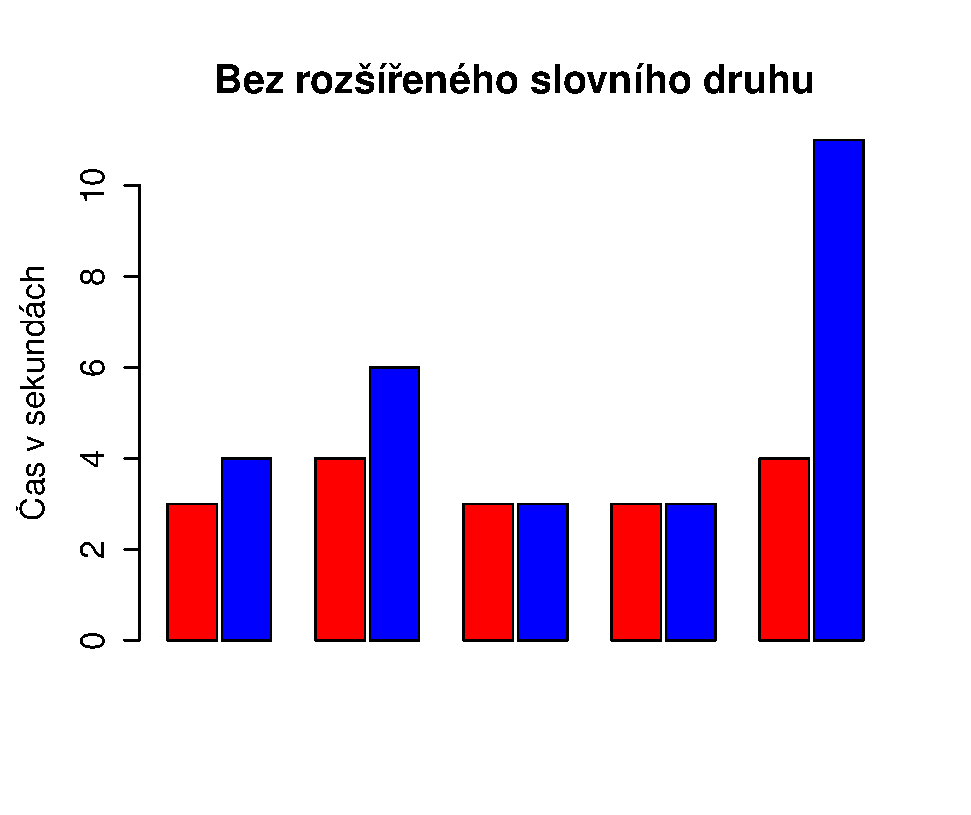
\includegraphics[width=70mm]{./grafy/morf/cas/rsd/bez.eps}
	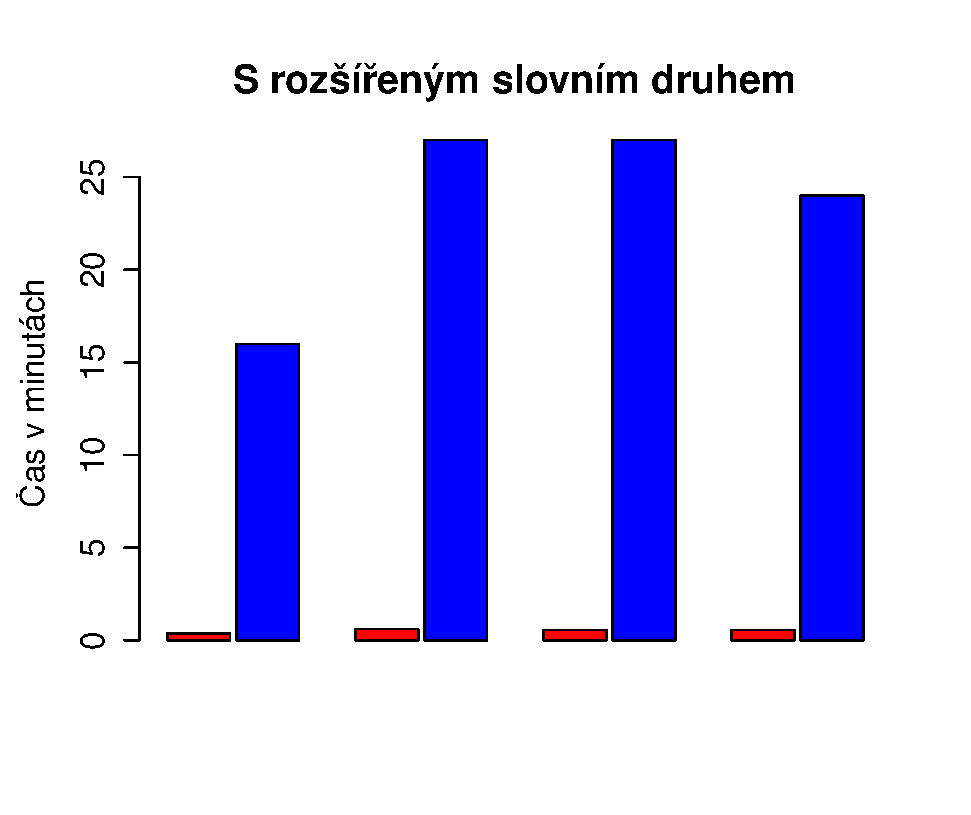
\includegraphics[width=70mm]{./grafy/morf/cas/rsd/rsd.eps}
\end{center}

\chapter{Modely s vlastní množinou rysů}
Problémy s německou gramatikou jsme se prozatím snažili řešit nahrazením slov morfologickými značkami. Modely s rozšířeným slovním druhem + morfologická analýza dopadly sice lépe než běžné modely trénované na slovech, přesto zlepšení není nijak výrazné. V následující kapitole se proto pokusíme upustit od n-gramů a postihnout gramatiku z jiné stránky - vlastní množinou rysů.

Trénovat už nebudeme ve SRILMu, neboť ten nepodporuje jiné než n-gramové rysy. Pro tyto modely použijeme maxent toolkit od LeZhanga\footnote{Lezhang}.

Pro následující experimenty jsme překladové hypotézy rozdělili na dva díly. Polovina tj. 1045 překladových hypotéz se použilo jako vývojová sada a druhá polovina jako sada testovací. Hypotézy byly rozděleny s ohledem na hodnocení plynulosti tak, aby vývojová i testovací množina vět obsahovala stejný počet hypotéz hodnocených plynulostí 1, 2, .., 5 (až na liché počty hypotéz některých plynulostí). Následující tabulka ukazuje přesné počty hypotéz a jejich rozdělení:

\begin{center}\begin{tabular}{|c|c|c|c|}
	\hline
	\textbf{Plynulost} & \textbf{Celkem hypotéz} & \textbf{Vývojová sada} & \textbf{Testovací sada}\\
	\hline
	1 & 150 & 75 & 75\\
	\hline
	2 & 445 & 222 & 223\\
	\hline
	3 & 932 & 466 & 466\\
	\hline
	4 & 387 & 194 & 193\\
	\hline
	5 & 176 & 88 & 88\\
	\hline
	\hline	
	\multicolumn{1}{c}{\textbf{CELKEM}} & \multicolumn{1}{c}{\textbf{2090}} & \multicolumn{1}{c}{\textbf{1095}} & \multicolumn{1}{c}{\textbf{1095}}\\
\end{tabular}\end{center}

\section{Zdrojová data}
\section{Způsob vyhodnocení}
\section{Princip experimentů}

\section{Vlastní rysy}
\section{JINÉ DĚLENÍ KAPITOL:}
\section{Modely se všemi rysy}
\section{Modely se všemi rysy kromě rysů součtových}
\subsection{Bez rysu root}
\section{Modely se součtovými rysy}
\subsection{S rysem root}
\section{Modely s rysem root}
\section{Modely s rysem sum}
\subsection{S rysem root}

\section{NAMÍSTO PŮVODNÍHO:}

\section{Počet kořenů v naparsovaném stromu}
Z gramaticky správné věty by měl jít vykreslit strom s větným rozborem. Předložíme-li ale ParZu větu, která správně není, vrátí nám stromů více.
%% TODO: doplnit priklady naparsovani vety s chybami
Zkusili jsme proto zjistit, jak spolu souvisí počet stromů z větného rozboru a ručně hodnocená plynulost překladu.
\begin{center}
	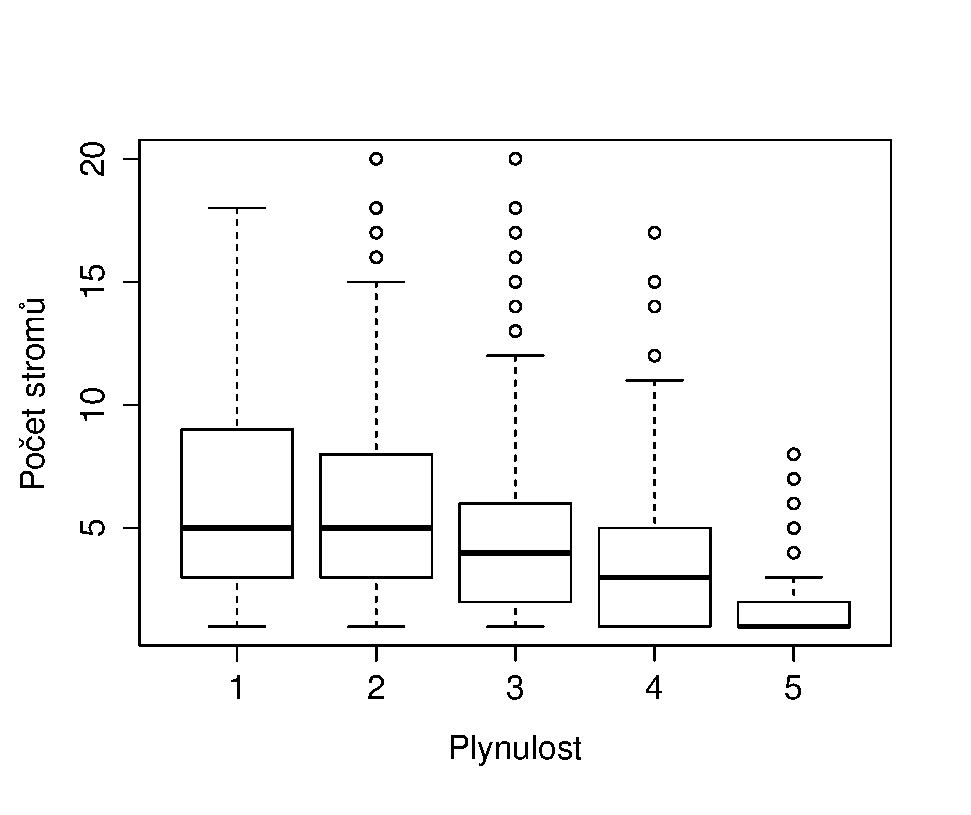
\includegraphics[width=70mm]{./grafy/pocet-stromu/pocet-stromu.eps}
\end{center}
Výsledky vypadají slibně, neboť boxploty mají výrazně klesavou tendenci. Je tedy patrné, že počet stromů z větného rozboru souvisí s ručně hodnocenou plynulostí.

\section{Chybějící infinitiv s zu}
\section{Chybějící podmět}
\section{Chybějící určité sloveso}
\section{Infinitiv po modálním slovese není na konci věty}
\section{Podmět se neshoduje s přísudkem}
\section{Příčestí minulé bez pomocného slovesa}
\section{Příčestí minulé není na konci věty}
\section{Jména a slovesa ve více osobách}
\section{Více určitých sloves ve větě}
\section{Určité sloveso není ve vedlejší větě na konci}
\section{Součtové rysy}

NAPSAT, ŽE SPOUSTU CHYB V PARZU ZAPŘÍČIŇUJE LOWERCASE!!! zahlen x Zahlen



% Ukázka použití některých konstrukcí LateXu (odkomentujte, chcete-li)
% %%% Ukázka použití některých konstrukcí LaTeXu

\subsection{Ukázka \LaTeX{}u}
\label{ssec:ukazka}

V~této krátké části ukážeme použití několika základních konstrukcí \LaTeX{}u,
které by se vám mohly při psaní práce hodit.

Třeba odrážky:

\begin{itemize}
\item Logo Matfyzu vidíme na obrázku~\ref{fig:mff}.
\item Tato subsekce má číslo~\ref{ssec:ukazka}.
\item Odkaz na literaturu~\cite{lamport94}.
\end{itemize}

Druhy pomlček:
červeno-černý (krátká),
strana 16--22 (střední),
$45-44$ (minus),
a~toto je --- jak se asi dalo čekat --- vložená věta ohraničená dlouhými pomlčkami.
(Všimněte si, že jsme za \verb|a| napsali vlnovku místo mezery: to aby se
tam nemohl rozdělit řádek.)

% Makro na české uvozovky (novější verze LaTeXu ho už mají zabudované)
\newcommand{\uv}[1]{\quotedblbase #1\textquotedblleft}
\uv{České uvozovky.}

\newtheorem{theorem}{Věta}
\newtheorem*{define}{Definice}	% Definice nečíslujeme, proto "*"

\begin{define}
{\sl Strom} je souvislý graf bez kružnic.
\end{define}

\begin{theorem}
Tato věta neplatí.
\end{theorem}

\begin{proof}
Neplatné věty nemají důkaz.
\end{proof}

\begin{figure}
	\centering
	
\includegraphics[width=30mm]{../img/logo.eps}
	\caption{Logo MFF UK}
	\label{fig:mff}
\end{figure}


\chapter*{Závěr}
\addcontentsline{toc}{chapter}{Závěr}


%%% Seznam použité literatury
%%% Seznam použité literatury je zpracován podle platných standardů. Povinnou citační
%%% normou pro bakalářskou práci je ISO 690. Jména časopisů lze uvádět zkráceně, ale jen
%%% v kodifikované podobě. Všechny použité zdroje a prameny musí být řádně citovány.

\def\bibname{Seznam použité literatury}
\addcontentsline{toc}{chapter}{\bibname}

\begin{thebibliography}{99}
%\addcontentsline{toc}{chapter}{\bibname}

%MUNROE, Randall. Random Number. In: XKCD: A webcomic of
%romance, sarcasm, math and language [online]. 2010
%[cit. 2011-10-04]. Dostupne z: ´ http://xkcd.com/221/

\bibitem{jurafsky08}
  {\sc JURAFSKY,} Dan a James {\sc H. MARTIN}. 
  \emph{Speech and language processing: an introduction to natural language processing, computational linguistics, and speech recognition}. 2nd ed. Upper Saddle River: Pearson Education, 2008. ISBN 978-0-13-187321-6. 



\bibitem{smrz06}
  {\sc SMRŽ,} Pavel. \emph{Jazykové modelování} [online]. 2006  [cit. 2013-05-04]. Dostupné z: \url{http://www.fit.vutbr.cz/study/courses/SRE/public/prednasky/2010-11/01_lm/SRE_LM.pdf}
  

\bibitem{fraser12}
  {\sc FRASER,} Alexander, Marion {\sc WELLER} a Cahilly Fabienne {\sc CAP}. \emph{Modeling Inflection and Word-Formation in SMT} 
  [online]. 2012
  [cit. 2013-05-04].
  Dostupné z: \url{http://eprints.pascal-network.org/archive/00009510/01/morphgen_hmm.pdf}  
 
  

\end{thebibliography}
 



%%% Tabulky v bakalářské práci, existují-li.
\chapwithtoc{Seznam tabulek}

%%% Použité zkratky v bakalářské práci, existují-li, včetně jejich vysvětlení.
\chapwithtoc{Seznam použitých zkratek}

%%% Přílohy k bakalářské práci, existují-li (různé dodatky jako výpisy programů,
%%% diagramy apod.). Každá příloha musí být alespoň jednou odkazována z vlastního
%%% textu práce. Přílohy se číslují.
\chapwithtoc{Přílohy}

\openright
\end{document}
